% 模板出处:https://zhuanlan.zhihu.com/p/379360037

\documentclass[12pt, a4paper, oneside]{book}
\usepackage{ctex}
\usepackage{amsmath, amsthm, amssymb, bm, graphicx, hyperref, mathrsfs, enumitem}
\hypersetup{
    colorlinks=true,
    linkcolor=blue,
    filecolor=blue,      
    urlcolor=blue,
    citecolor=cyan,
}
\usepackage{pgfplots}
\pgfplotsset{compat=newest}
\usepackage{comment}
\usepackage{titlesec,titleps} % 添加 titlesec 宏包
\titleclass{\section}{straight} % 清除默认章节格式

% 章节格式统一设置
\titleformat{\section}[runin]
  {\normalfont\bfseries}
  {\thesection.}
  {-0.5em}
  {\quad}
  
\titleformat{\subsection}[runin]
  {\normalfont\bfseries}
  {\thesubsection.}
  {-0.3em}
  {\quad}

% 间距微调
\titlespacing*{\section}
  {0pt}
  {1.2ex plus 0.5ex minus 0.2ex}
  {0.3em}

\titlespacing*{\subsection}
  {15pt} % 二级标题增加缩进
  {0.8ex plus 0.3ex minus 0.1ex}
  {0.2em}

\renewcommand{\thesection}{\arabic{section}}
\renewcommand{\thesubsection}{\arabic{section}\arabic{subsection}}

% 图编号格式调整
\numberwithin{figure}{section}

% 定理环境样式调整
\theoremstyle{definition}
\newtheorem{theorem}{定理}[section]
\newtheorem{lemma}[theorem]{引理}
\newtheorem{definition}[theorem]{定义}
\newtheorem{example}[theorem]{例}
\newtheorem{proposition}[theorem]{命题}

% 页眉页脚设置(来自于 titleps 宏包)
% 设置页眉为楷体
\newpagestyle{main}{
    \sethead{\kaishu \sectiontitle}{}{\kaishu \thepage}
}
\pagestyle{main}

\title{{\Huge{\textbf{测度与概率 Notes}}}}
\author{Liu Fuzhou}
\date{\today}
\linespread{1.5}






\begin{document}

\maketitle

\pagenumbering{roman}
\setcounter{page}{1}

%\begin{comment}
\begin{center}
    \Huge\textbf{前言}
\end{center}~\

要看偏微分方程,就要先看泛函分析. 要看泛函分析,就要先看实分析. 泛函分析和实分析对随机分析也是重要的. 无论如何也绕不开 $L^p$ 空间. 可见掌握实分析十分重要. 以前其实也看过这个主题的书,结果后来都忘了. 看来做一些有形的笔记是很有必要的. 不需要特别详细,提纲挈领即可.

主要参考文献:
\begin{enumerate}
\item[1.] 近代概率引论:测度、鞅和随机微分方程. 袁震东. 科学出版社, 1991.
\item[2.] 测度与概率教程. 任佳刚,巫静. 科学出版社, 2018.
\item[3.] Measure, Integration \& Real Analysis. Sheldon Axler. Springer, 2020.
\end{enumerate}

~\\
\begin{flushright}
    \begin{tabular}{c}
        Liu Fuzhou\\
        \today
    \end{tabular}
\end{flushright}
%\end{comment}

\newpage
\pagenumbering{Roman}
\setcounter{page}{1}
\tableofcontents
\newpage
% 生成图表目录
\listoffigures
\newpage
\setcounter{page}{1}
\pagenumbering{arabic}


\section{集列的极限}
首先比较重要的概念就是集列的上极限与下极限. 集列 $\{A_n\}_{n\in\mathbb N}$ 的上极限就是落到其中无限多个集合的元素所做成的集合,也即 $\limsup_{n\to\infty}A_n=\bigcap_{n=1}^\infty\bigcup_{k=n}^\infty A_k.$ 
下极限就是除去有限多个集合后,落到所有集中的元素所做成的集合,也即 $\liminf_{n\to\infty}A_n=\bigcup_{n=1}^\infty\bigcap_{k=n}^\infty A_k.$ 换言之也即“最终落到集列” $A_n$ 中的那些元素之全体.
显然,下限集中的元素也都落到上限集之中,也即 $\liminf A_n\subset \limsup A_n.$ 如果集列 $A_n$ 的上限集与下限集相等,那么就说集列 $A_n$ 收敛,并称 $A=\liminf A_n=\limsup A_n$ 为集列 $A_n$ 的极限. 这个极限是关于集合包含的偏序关系说的. 
与实数的情况类似,有单调集列的收敛定理:如果 $A_n\uparrow$ 是单调递增的,那么 $\lim A_n=\bigcup_n A_n.$ 类似地,如果 $A_n\downarrow$ 是单调递减的,那么 $\lim A_n=\bigcap_n A_n.$ 


\begin{example}
    设 $\{A_n\}_{n\in\mathbb N}$ 为单调减少集列. 证明 
    \begin{equation*}
        A_1=\sum_{n=1}^\infty (A_n-A_{n+1}) + \bigcap_{n=1}^\infty A_n
    \end{equation*}
\end{example}
\begin{proof}
首先,右边的每个集合都含于 $A_1.$ 因此右边含于 $A_1.$ 其次,若 $x\in A_1$ 且 $x\notin \bigcap_{n=1}^\infty A_n$, 则 $x\in \sum_{n=1}^\infty (A_n-A_{n-1})$ 且 $x\notin \bigcap_{n=1}^\infty A_n.$ 因此 $A_1$ 也是单调递减的. 最后,若 $x\in \bigcap_{n=1}^\infty A_n$, 则存在某个 $n>1,$ 使得 $x\notin A_n.$ 令 $n_0$ 为最小的这种 $n,$ 那么就有 $x\notin A_{n_0},\ x\in A_{n_0-1}.$ 于是就有 $x\in \sum_{n=1}^\infty (A_n-A_{n-1}).$ 这就证明了 
$A_1\subset \sum_{n=1}^\infty (A_n-A_{n+1}) + \bigcap_{n=1}^\infty A_n.$ 
\end{proof}

\section{Riemann 积分} 
还是用 \cite{Axler_2020} 作为参考书比较好,还是彩色的. 我还是比较喜欢 Riemann 积分的,最开始是在梅加强的书上学的. 比较重要的技术就是证明 Darboux 上和总是大于等于 Darboux 下和那里,需要用到两个 partition 的 merge. 也就是说,用到了有界闭区间的 partition 全体构成一个 directed set 的性质. Darboux 上和与 Darboux 下和之差就是所谓的函数振幅 
$\Omega_\mathcal P (f)=\sum_{i} (\sup_{x_{i-1}\leq x\leq x_i} f-\inf_{x_{i-1}\leq x\leq x_i})(x_i-x_{i-1}),$ 这里 $\mathcal P=\{a=x_0<x_1<\cdots<x_n=b\}$ 是所讨论的具体的分割. 

如果向 partition 的点集增加元素,也即使得分割变得更细,那么结果就是上和不增,下和不减. 这就导致了两个极限 $\lim_{\mathcal P} \mathcal L(f,\mathcal P,[a,b])$ 和 $\lim_{\mathcal P} \mathcal U(f,\mathcal P,[a,b]),$ 称为 Riemann 下积分 $\underline{\int}$ 和上积分 $\overline{\int}$. 这两个极限是关于 partition 全体所具有的 directed set 结构说的, 也就是说是 net 的极限. 由于下和不大于上和,也即 $\mathcal L\leq \mathcal U,$ 因此这两个极限之间也有关系
\begin{equation}
    \underline{\int}_a^b f(x)\ \mathrm dx\leq  \overline{\int}_a^b f(x)\ \mathrm dx
\end{equation}
如果 Riemann 上下积分相等,就说 $f$ 在 $[a,b]$ 上 Riemann 可积,其积分 $\int_a^b f(x)\ \mathrm dx$ 就定义为上下积分的共同值. 

任意分割 $\mathcal P$ 都将区间 $[a,b]$ 分成 $\#(\mathcal P)-1$ 个首尾相接的闭区间 $[x_0,x_1],\cdots,[x_{n-1},x_n].$ 从每个闭区间挑选一个元素出来,就可以做成一个集合 $\Delta.$ 这种挑选当然是不唯一的. 称这种通过在每个闭区间中挑出一个元素所形成的集合为与 partition $\mathcal P$ 相伴的一个点集. 
设 $\{\mathcal P_n\}_{n\in\mathbb N}$ 是任意一列 partition, 并且 $\{\Delta_n\}_{n\in\mathbb N}$ 是一列与之相伴的点集,每个 $\Delta_n$ 中元素形如 $\Delta_n=\{\xi_1,\cdots,\xi_{\#(\mathcal P_n)-1}\},$ 那么就可以考虑 Riemann 和所形成的数列
\begin{equation}
    \mathcal R_n:=\mathcal R(f,\mathcal P_n,\Delta_n,[a,b])=\sum_{i=1}^{\#(\mathcal P_n)-1} f(\xi_i)(x_{i}-x_{i-1})
\end{equation}
显然有 $\mathcal L(f,\mathcal P_n,[a,b])\leq \mathcal R_n\leq \mathcal U(f,\mathcal P_n,[a,b]).$ 因此有
\begin{equation}\label{eq:Riemann limit inequalities}
    \underline{\int}_a^b f(x)\ \mathrm dx\leq \liminf \mathcal R_n\leq \limsup \mathcal R_n\leq  \overline{\int}_a^b f(x)\ \mathrm dx
\end{equation}

这就表明,如果 $\mathcal R_n$ 有收敛子列的话,那么该子列的极限就必定位于上下积分之间.  当然了,如果 $f$ 是 Riemann 可积的,这个极限就必定等于 $\int_a^b f(x)\ \mathrm dx.$ 


以上讨论了利用 partition 的全体所组成的集合之上的 directed set 结构来定义的 Riemann 积分. 下面考虑利用 Riemann 和关于 partition 的 mesh 的极限的途径. 这就是说,把 Riemann 积分定义为极限
\begin{equation}\label{eq:Riemann_limit}
    \lim_{\|\mathcal P\|\to 0} \mathcal R(f,\mathcal P,\Delta,[a,b])
\end{equation}
其中 $\|\mathcal P\|=\max_{i}|x_{i}-x_{i-1}|$ 是 partition 的 mesh. 这个极限其实相当强,因为其定义只涉及 partition, 对相伴的点集 $\Delta$ 没什么要求.  

由不等式 \eqref{eq:Riemann limit inequalities} 可知,如果两种定义下的 Riemann 积分均存在,那么它们的值必定相等. 因此,两种定义的等价性的证明就归结于证明其存在性的等价性.


要证明两种定义的等价性,首先要注意到,上下积分之差恰好等于函数振幅的下确界 $\inf_{\mathcal P}\Omega_\mathcal P(f).$ 这就是说 $\lim_{\mathcal P} (\mathcal U(f,\mathcal P,[a,b])-\mathcal L(f,\mathcal P,[a,b]))=\inf_{\mathcal P}\Omega_\mathcal P(f),$ 或者说 $\lim_{\mathcal P}\Omega_\mathcal P(f)=\inf_{\mathcal P}\Omega_\mathcal P(f).$ 
事实上,设 $\varepsilon>0,$ 那么由 net 的极限的定义,存在 partition $\mathcal P_0,$ 使得任意细于 $\mathcal P_0$ 的分割 $\mathcal P$ 都满足 $|\Omega_{\mathcal P_0}(f)-\lim_{\mathcal P} \Omega_{\mathcal P}(f)|<\varepsilon.$ 
另一方面,由下确界的定义,存在 partition $\mathcal P_1$ 使得 $\Omega_{\mathcal P_1}(f)< \inf_{\mathcal P}\Omega_{\mathcal P}(f)+\varepsilon.$
取分割 $\mathcal P_2$ 为 $\mathcal P_0$ 与 $\mathcal P_1$ 的 merge, 那么就有 
\begin{equation}
    \lim_{\mathcal P}\Omega_{\mathcal P}(f)-\varepsilon< \Omega_{\mathcal P_2}(f)\leq \Omega_{\mathcal P_1}(f)<\inf_{\mathcal P}\Omega_{\mathcal P}(f)+\varepsilon
\end{equation}
于是 $\inf_{\mathcal P}\Omega_{\mathcal P}(f)\leq \lim_{\mathcal P}\Omega_{\mathcal P}(f)<\inf_{\mathcal P}\Omega_{\mathcal P}(f)+2\varepsilon.$ 这就证明了 
\begin{equation}
    \overline{\int}_a^b f(x)\ \mathrm dx - \underline{\int}_a^b f(x)\ \mathrm dx = \inf_{\mathcal P}\Omega_{\mathcal P}(f)
\end{equation}

假如极限 \eqref{eq:Riemann_limit} 存在,其值记为 $A,$ 那么对于任意的 $\varepsilon>0,$ 存在 $\delta>0,$ 使得只要 partition 的 mesh 小于 $\delta,$ 就有 $|\mathcal R(f,\mathcal P,\Delta,[a,b])-A|<\varepsilon.$ 
现在固定分割 $\mathcal P,$ 那么由于该不等式对于任意与 $\mathcal P$ 相伴的点集 $\Delta$ 都成立,因此有 $\Omega_{\mathcal P}(f)\leq 2\varepsilon.$ 这就证明了 $\inf_{\mathcal P}\Omega_{\mathcal P}(f)=0,$ 因而上下积分相等. 

反之,要从上下积分相等导出极限 \eqref{eq:Riemann_limit} 的存在性,还需要证明一个基于 partition 的 mesh 估计的技术性引理:
\begin{lemma}\label{lemma:mesh estimate}
    设 $\mathcal P,\mathcal P'$ 为区间 $[a,b]$ 的两个 partition, $M=\sup_{x\in [a,b]}|f(x)|,$ 那么就有不等式 
    \begin{equation}\label{eq:mesh estimate}
        \Omega_{\mathcal P}(f) \leq \Omega_{\mathcal P'}(f) + (\#(\mathcal P')-2)M\|\mathcal P\|
    \end{equation}
\end{lemma}

事实上,如果向 $\mathcal P$ 中添加一个新元素 $y,$ 譬如说插入到区间 $[x_k,x_{k+1}]$ 中,那么所形成的新分割 $\mathcal P''$ 的 Darboux 和与 $\mathcal P$ 的 Darboux 的差异仅来自于区间 $[x_k,x_{k+1}]$ 的贡献,也即
\begin{equation}
    \Omega_{\mathcal P''}(f)-\Omega_{\mathcal P}(f)=\omega_{x_k\leq x\leq y}f(x) (y-x_k)+ \omega_{y\leq x\leq x_{k+1}}f(x) (x_{k+1}-y) - \omega_{x_k\leq x\leq x_{k+1}}f(x) (x_{k+1}-x_k)
\end{equation}
考虑到 $\omega_{x_k\leq x\leq y}-\omega_{x_k\leq x\leq x_{k+1}}$ 和 $\omega_{y\leq x\leq x_{k+1}}-\omega_{x_k\leq x\leq x_{k+1}}$ 都落到区间 $[-M,M]$ 内,因此 $\Omega_{\mathcal P''}(f)-\Omega_{\mathcal P}(f)$ 的绝对值被 $M(x_{k+1}-x_k)$ 控制, 
从而也被 $M\|\mathcal P\|$ 控制. 这就导出了 $|\Omega_{\mathcal P''}(f)-\Omega_{\mathcal P}(f)|\leq M\|\mathcal P\|.$ 类似地,如果向 $\mathcal P''$ 中再插入一个新元素得到新分割 $\mathcal P''',$那么同样有
\begin{equation}
    |\Omega_{\mathcal P'''}(f)-\Omega_{\mathcal P''}(f)|\leq M\|\mathcal P''\|
\end{equation}
由于 $\mathcal P'''$ 细于 $\mathcal P,$ 因此 $\|\mathcal P'''\|\leq \|\mathcal P\|.$ 因此 $\Omega_{\mathcal P'''}(f)-\Omega_{\mathcal P''}(f)$ 的绝对值也被 $M\|\mathcal P\|$ 控制,从而有 $|\Omega_{\mathcal P'''}(f)-\Omega_{\mathcal P}(f)|\leq 2 M\|\mathcal P\|.$ 
现在考虑 $\mathcal P$ 与 $\mathcal P'$ 的 merge $\mathcal S,$ 其可以通过反复向 $\mathcal P$ 中插入元素来得到,插入次数至多为 $ \#(\mathcal P')-2$ 次. 因此就有
\begin{equation}
    \Omega_{\mathcal P}(f)-(\#(\mathcal P')-2)M\|\mathcal P\|\leq \Omega_{\mathcal S}(f)\leq \Omega_{\mathcal P'}(f)
\end{equation}
这就导出了不等式 \eqref{eq:mesh estimate}. 这个引理最初是在 \cite{Mei_2011} pp.213 看到的.

作为引理 \ref{lemma:mesh estimate} 的一个推论,立刻可以导出
\begin{equation}\label{eq:Riemann_limit_mesh_inf}
    \lim_{\|\mathcal P\|\to 0} \Omega_{\mathcal P}(f)=\inf_{\mathcal P}\Omega_{\mathcal P}(f)
\end{equation}
这是因为,设 $\varepsilon>0,$ 那么由下确界的定义可知存在 partition $\mathcal P_0,$ 使得 $\Omega_{\mathcal P_0}(f)<\inf_{\mathcal P}\Omega_{\mathcal P}(f)+\varepsilon.$ 
记 $N=\#(\mathcal P_0)-2,$ 那么当 partition 的 mesh 小于 $\varepsilon/(MN)$ 时,由引理 \ref{lemma:mesh estimate} 可知
\begin{equation}
    \Omega_{\mathcal P}(f)\leq\Omega_{\mathcal P_0}(f)+(\#(\mathcal P')-2)M\|\mathcal P\|<\inf_{\mathcal P}\Omega_{\mathcal P}(f)+2\varepsilon
\end{equation}
这就证明了 \eqref{eq:Riemann_limit_mesh_inf} 式. 类似地可以证明
\begin{equation}\label{eq:Riemann_limit_mesh_upper_lower}
    \lim_{\|\mathcal P\|\to 0} \mathcal L(f,\mathcal P,[a,b])=\underline{\int}_a^b f(x)\ \mathrm dx,\ \lim_{\|\mathcal P\|\to 0} \mathcal U(f,\mathcal P,[a,b])=\overline{\int}_a^b f(x)\ \mathrm dx.
\end{equation}

现在假设 Riemann 上下积分相等,也即 $\lim_{\|\mathcal P\|\to 0}\Omega_{\mathcal P}(f)=0,$ 那么对于任意的 $\varepsilon>0,$ 存在 $\delta>0,$  使得只要 partition 的 mesh 小于 $\delta,$ 就有
$|\mathcal U-\overline{\int}|,|\mathcal L-\underline{\int}|< \varepsilon.$ 自然,此时由不等式 \eqref{eq:Riemann_limit_mesh_upper_lower} 可知
\begin{equation}
    \underline{\int}_a^b f(x)\ \mathrm dx-\varepsilon<\mathcal L(f,\mathcal P,[a,b])\leq \mathcal R(f,\mathcal P,\Delta,[a,b])\leq \mathcal U(f,\mathcal P,[a,b])\leq \overline{\int}_a^b f(x)\ \mathrm dx+\varepsilon
\end{equation}
这就证明了极限 \eqref{eq:Riemann_limit} 的存在性.

容易验证闭区间上的连续函数是 Riemann 可积的. 这主要用到了其一致连续性.

\section{Riemann 积分的若干缺陷}\label{sec:deficiencies_of_Riemann_integral}

Riemann 积分的一些缺陷:
\begin{enumerate}
    \item 如果函数的连续性较差,则其 Riemann 可积性也较差:典型的例子就是 Dirichlet 函数.
    \item 无界函数的 Riemann 可积性较差(反常积分):一个例子就是取一列可求出瑕积分的函数 $f_k(x),$ 使得每个函数的瑕点恰好对应区间 $[0,1]$ 上的一个有理数,最终导致无法通过划分区间的办法求出函数 $f:=\sum_k {f_k\over 2^k}$ 的瑕积分. 这里其实是说,
          如果将面积的次可加性推广到可数的情况,那么通常的 Riemann 积分就不太够用了. 毕竟这样构造出的 $f$ 多多少少是个较为奇怪的函数,这种例子更偏向于理论意义. 
    \item Riemann 积分与极限的可交换性较差:这个问题看起来是最为致命的. 可以构造出一列函数 $f_k,$ 它们的 Riemann 积分均为零,但其逐点收敛到 Dirichlet 函数. 虽然可以证明,如果一致有界的可积函数列的逐点极限函数是 Riemann 可积的,那么其积分与极限可以交换位置,也即 $\lim_{n} \int_a^b f_n = \int_a^b \lim_n f_n,$ 但其证明 
          却非常复杂,并且也绕不过使用测度的思想. 这个缺陷使得 Riemann 积分在理论上使用起来尤为不便. 
\end{enumerate}

\begin{example}
    定义闭区间 $[0,1]$ 上的函数 $f$ 为
    \begin{equation}
        f(x)=\begin{cases}
            0, & \text{若 $x$ 为无理数}\\
            {1\over n}, & \text{若 $x$ 为有理数,且 $n$ 为形如 $x={m\over n}$ 的表达式中的最小正整数 $n$}
        \end{cases}
    \end{equation}
    证明 $f$ 是 Riemann 可积的,并计算其积分值.
\end{example}
显然 $f$ 的每一个 Darboux 下和都为零,因此 $\underline{\int}_0^1 f = 0.$ 下面证明 $f$ Riemann 可积. 只需构造出一列 partition $\mathcal P_n,$ 使得 $\lim_n \Omega_{\mathcal P_n}(f)=0$ 即可. 由于 $\mathcal L\equiv 0,$ 因此只需证明 $\lim_n \mathcal U(f,\mathcal P_n,[0,1])=0.$
事实上,对于任意的 $n,$ 满足 $f(x)=1/n$ 的 $[0,1]$ 内的有理数至多有 $n+1$ 个,因此其数目有限. 自然,可以适当地划分区间,得到分割 $\mathcal P_n,$ 使得满足 $f(x)\geq 1/n,$ 也即 $f(x)=1,1/2,\cdots,1/n$ 的全体有理数 $x$ 所在的区间的总长不超过 $1/n.$ 自然,$f$ 在剩下的那些区间上的上确界均小于 $1/n.$ 于是就有
\begin{equation}
    \begin{aligned}
        \mathcal U(f,\mathcal P_n,[0,1])=&\sum_{\text{$f(x)\geq 1/n$ 的 $x$ 所在区间 $[x_{i-1},x_{i}]$}} \sup_{x_{i-1}\leq x\leq x_i}f(x)(x_i-x_{i-1})\\
        &+\sum_{\text{其余区间 $[x_{i-1},x_{i}]$}}\sup_{x_{i-1}\leq x\leq x_i}f(x)(x_i-x_{i-1})  \\
        <& {1\over n}-{1\over n}\left(1-{1\over n}\right) \\
        =&{2\over n}-{1\over n^2}
    \end{aligned}
\end{equation}
于是就有 $\lim_n \mathcal U(f,\mathcal P_n,[0,1])=0.$ 因此 $f$ 是 Riemann 可积的,并且其 Riemann 积分为 $\int_0^1 f=0.$


\begin{example}
    Riemann 积分与极限交换时,一致有界条件不可去掉.
\end{example}
事实上,构造单位区间 $[0,1]$ 上的连续函数列
\begin{equation}\label{eq:swap_limit_counterexample}
    f_n(x) = \begin{cases}
        n^2 x, & \text{若 $0\leq x\leq 1/n$}\\
        2n-n^2x, & \text{若 $1/n<x\leq 2/n$}\\
        0&\text{若 $x>2/n$}
    \end{cases}
\end{equation}

\begin{figure}[]
    \centering
    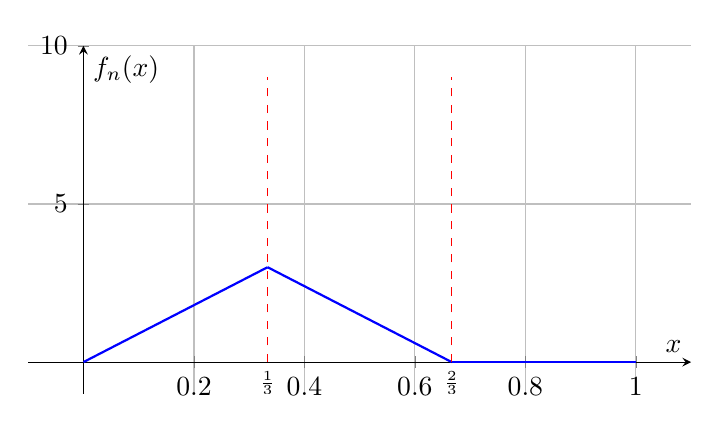
\begin{tikzpicture}
    \begin{axis}[
        axis lines = middle,
        xlabel = {$x$},
        ylabel = {$f_n(x)$},
        ymin = -1, ymax = 10,
        xmin = -0.1, xmax = 1.1,
        domain = 0:1,
        samples = 100,
        grid = major,
        width=10cm,
        height=6cm,
    ]
    
    % Define n
    \def\n{3}
    
    % Plot the function
    \addplot [thick, blue, domain=0:1/\n] {(\n)^2 * x};
    \addplot [thick, blue, domain=1/\n:2/\n] {2*\n - (\n)^2 * x};
    \addplot [thick, blue, domain=2/\n:1] {0};
    
    % Add vertical lines at x = 1/n and x = 2/n
    \draw [dashed, red] (axis cs:1/\n,0) -- (axis cs:1/\n,9);
    \draw [dashed, red] (axis cs:2/\n,0) -- (axis cs:2/\n,9);
    
    % Add labels for the vertical lines
    \node [below, font=\scriptsize] at (axis cs:1/\n,0) {$\frac{1}{3}$};
    \node [below, font=\scriptsize] at (axis cs:2/\n,0) {$\frac{2}{3}$};
    
    \end{axis}
    \end{tikzpicture}
    \caption{Graph of the piecewise function \( f_n(x) \) depicted by equation \eqref{eq:swap_limit_counterexample} for \( n=3 \).}
    \label{fig:fn}
\end{figure}

那么就有 $\int_0^1 f_n = 1,$ 以及 $\lim_n f_n(x)\equiv 0.$ 这是因为 $f_n(x)$ 也就只在开区间 $(0,2/n)$ 上不为零,该区间随着 $n\to\infty$ 而消失.
因此,极限函数 $f:=\lim_n f_n$ 是连续的,并且有 $\int_0^1 f=0.$ 因此
\begin{equation}
    \lim_n \int_0^1 f_n = 1\neq 0=\int_0^1 \lim_n f_n
\end{equation}
当然,$f_n$ 不是一致有界的:$\sup_{x\in [0,1]}f_n(x)=n,$ 因此 $f_n(x)$ 不可能被某个有限的数所一致控制.


\section{外测度} 外测度的概念是经典的:对 $\mathbb R$ 的任意子集 $A,$ 都可定义其外测度 $|A|$ 为覆盖 $A$ 的开区间列的总长度之下确界,也即 $|A|=\inf_{A\subset\bigcup_n I_n} \sum_n \ell(I_n).$
这总是定义良好的. 如果某个 $\ell(I_n)$ 为 $+\infty,$ 那么显然 $\sum_n \ell(I_n)=+\infty.$ 反之,$\sum_n \ell(I_n)$ 是一个非负项的数项级数. 
自然,非负项级数要么收敛,要么发散到 $+\infty.$ 因此,如果将 $+\infty$ 也作为一个合法的长度值,
那么 $\sum_n \ell(I_n)$ 总是有定义的,并且总是大于等于零. 因此任意的实数集 $A$ 的外测度总是有定义的.

\begin{example}
    可数集的外测度为零.
\end{example}
设 $A=\{a_n\}_{n\in\mathbb N},\ \varepsilon>0,$ 那么可以构作区间列 $I_n=(a_n-\varepsilon/2^n,a_n+\varepsilon/2^n),$ 使得 $A\subset \bigcup_n I_n,$ 于是 
\begin{equation}
    |A|\leq \sum_n \ell(I_n)=\sum_n {\varepsilon\over 2^{n-1}}=2\varepsilon
\end{equation}
这就证明了 $|A|=0.$ 

特别地,有理数集 $\mathbb Q$ 的外测度为零. 这表明外测度的性质至少要比 Jordan 测度要好,因为 $\mathbb Q\cap [0,1]$ 的 Jordan 测度正是 Dirichlet 函数的 Riemann 积分,因而是不存在的.

如果实数集 $A$ 含于 $B,$ 那么任意覆盖了 $B$ 的开区间列也覆盖了 $A,$ 因而 $|A|\leq |B|.$ 因此外测度与集合的包含关系的相容性良好. 此外,由于平移变换并不改变开区间的长度,并且将开区间变为开区间,并且还是可逆的,因此任意实数集 $A$ 平移 $t$ 距离后,其外测度保持不变:$|A+t|=|A|.$ 这就是说外测度具有平移不变性.

外测度最为重要的一条性质恐怕就是次可数可加性了.
\begin{theorem}
    外测度具有次可数可加性:$|\bigcup_n A_n|\leq \sum_n |A_n|.$
\end{theorem}
首先,如果某个集合 $A_n$ 的外测度为 $+\infty,$ 那么结论显然成立. 下面假设所有 $|A_n|$ 都是有限的. 设 $\varepsilon>0.$ 对于任意固定的 $n,$ 根据外测度的定理,可以找到一列开区间 $\{I_{n,k}\}_{k\in\mathbb N},$ 使得
\begin{equation}
    \sum_k \ell(I_{n,k})<|A_n|+{\varepsilon\over 2^n}
\end{equation}
自然,记所有这些区间 $I_{n,k}$ 所做成的集合为 $X,$ 那么映射 $\mathbb N\times\mathbb N\to X,\ (n,k)\mapsto I_{n,k}$ 可以重新排列顺序为 $\mathbb N\to X,\ j\mapsto I_{n(j),k(j)}.$ 这一列区间 $I'_j:=I_{n(j),k(j)}$ 覆盖了 $\bigcup_n A_n,$ 并且对于每个正整数 $p\in\mathbb N,$ 记 $n(1),\cdots,n(p)$ 中的最大值为 $N(p),$ 则有
\begin{equation}
    \sum_{j=1}^p \ell(J_j) \leq \sum_{n=1}^{N(j)} \sum_k \ell(I_{n,k}) \leq \sum_n\sum_k \ell(I_{n,k})<\sum_n |A_n|+\varepsilon
\end{equation}
于是 $\sum_j \ell(J_j)\leq\sum_n |A_n|+\varepsilon.$ 
这就证明了 
\begin{equation}\label{eq:outer_measure_subadditivity}
    \left|\bigcup_n A_n\right|\leq \sum_n |A_n|
\end{equation}
作为一个简单推论,外测度也具有次有限可加性:$|A_1\cup\cdots\cup A_n|\leq \sum_{i=1}^n |A_i|.$ 

下面来计算有界区间的外测度. 从几何上来看,开区间 $(a,b)$ 的外测度应该就等于其长度 $b-a.$ 严格的证明稍微麻烦一些,需要借助有界闭区间的紧性. 首先,$(a,b)$ 与 $[a,b]$ 的外测度相同:$|(a,b)|\leq |[a,b]|\leq b-a,$ 并且由 $[a,b]\subset (a-\varepsilon,b+\varepsilon),$ 以及 
$|(a-\varepsilon,b+\varepsilon)|\leq |(a,b)|+2\varepsilon$ 可得 $[a,b]\leq (a,b).$ 这就证明了开区间 $(a,b)$ 的外测度与其闭包相同. 另一方面,由 $[a,b]$ 的紧性可知,任意覆盖了 $[a,b]$ 的开区间列 $I_n$ 都存在有限子覆盖 $J_1,\cdots,J_p.$ 
下面只需证明 $\sum_{i=1}^p \ell(J_i)\geq b-a$ 即可. 最简单的证法是用归纳法(\cite{Axler_2020} pp. 20). 当 $p=1$ 时结论显然成立. 假设该结论对 $p\leq k$ 成立,那么当 $p=k+1$ 时,设 $[a,b]$ 被开区间 $J_1,\cdots,J_p$ 中的某个 $J_s=(c,d)$ 所覆盖,那么若 $c\leq a,$ 则 $\ell((c,d))\geq b-a,$ 故结论成立. 
若 $c>a,$ 则闭区间 $[a,c]$ 被 $k$ 个开区间 $\{J_i\}_{1\leq i\leq p,\ i\neq s}$ 所覆盖,于是由归纳假设即知 $\sum_{i\neq s}\ell(J_i)\geq c-a.$ 于是就有 $\sum_{i=1}^p \ell(J_i)\geq (c-a)+(b-c)=b-a,$ 因此总是有 
$\sum_n \ell(I_n)\geq b-a.$ 这就证明了 $|[a,b]|=b-a,$ 因而开区间 $(a,b)$ 的外测度也等于 $b-a.$

利用区间的外测度还可以给出区间的不可数性的另一个证明.
\begin{example}
    非空区间是不可数的.
\end{example}
事实上,由于可数集的外测度为零,而非空区间的外测度都大于零,因而非空区间不可能是可数集. 这就证明了结论.

\section{外测度的缺点:不可加性} Vitali 提供了集合的不交并的外测度不等于各自外测度之和的一个例子. 
\begin{example}[Vitali]\label{ex:non_additivity_of_outer_measure}
    存在不交的实数集 $A$ 和 $B$,使得 $|A\cup B|\neq |A|+|B|.$
\end{example}
对于区间 $[-1,1]$ 内的任意实数 $a,$ 定义相伴的集合 $\tilde a$ 为 $[-1,1]$ 内所有与 $a$ 只相差一个有理移位的元素之全体,那么若 $\tilde a\cap\tilde b\neq \emptyset,$ 譬如说 $c\in\tilde a\cap\tilde b,$ 那么就有 
$a-c,b-c\in\mathbb Q.$ 因此 $a,b$ 本身就只相差一个有理移位. 因此对于任意实数来说,与 $a$ 的距离为有理数当且仅当与 $b$ 的距离为有理数,从而有 $\tilde a=\tilde b.$ 
自然,由 $a\in\tilde a$ 可知 $[-1,1]\subset \bigcup_{a\in [-1,1]}\tilde a.$ 利用选择公理可从集合簇 $\{\tilde a\}_{a\in [-1,1]}$ 中的每个集合中取出一个元素,做成一个新集合 $V.$ 令 $[-2,2]$ 内的全体有理数所做成的数列为 $r_1,r_2,\cdots,$ 
那么就有 $[-1,1]\subset\bigcup_{k} (r_k+V).$ 这是因为对于 $[-1,1]$ 中的任意元素 $a,$ 设 $V$ 所含的 $\tilde a$ 中元素为 $x,$ 则有 $a-x\in\mathbb Q\cap [-2,2],$ 因而 $a-x$ 等于某个 $r_k,$ 于是 $a\in \bigcup_{k} (r_k+V).$ 
由外测度的次可数可加性和平移不变性即知
\begin{equation}
    2=|[-1,1]|\leq\sum_k |r_k+V|=\sum_k |V|
\end{equation}
这表明 $V$ 的外测度必定大于零. 容易验证集列 $\{r_k+V\}_{k\in\mathbb N}$ 是互不相交的. 这是因为,若 $x\in (r_{k_1}+V)\cap (r_{k_2}+V),$ 其中 $r_{k_1}\neq r_{k_2},$ 那么存在实数 $a,b,$ 使得 $x-r_{k_1}\in \tilde a\cap V,\ x-r_{k_2}\in\tilde b\cap V.$ 自然,$x-r_{k_2}=x-r_{k_1}+(r_{k_1}-r_{k_2})$ 也落入 $\tilde a$ 中,这就表明 $\tilde a$ 与 $\tilde b$ 相交,于是 $\tilde a=\tilde b.$ 由 $V$ 的定义即知 $x-r_{k_1}=x-r_{k_2},$ 这就导出了 $r_{k_1}=r_{k_2},$ 矛盾!

由于 $r_k\in [-2,2],\ V\subset [-1,1],$ 因此 $\bigcup_k (r_k+V)\subset [-3,3].$ 于是 $|\bigcup_k (r_k+V)|\leq 6.$ 另一方面,由于 $|V|>0,$ 因此必定存在 $n\in\mathbb N,$ 使得 
\begin{equation}
    \left|\bigcup_{k=1}^n (r_k+V)\right|< n|V|=\sum_{k=1}^n |r_k+V|
\end{equation}
特别地,如果对于任意的不交的实数集 $A,B,$ 均有等式 $|A\cup B|=|A|+|B|,$ 那么以上不等式必定不成立. 因此必定存在不交的集合 $A,B,$ 使得其并集的外测度不等于各自外测度之和.

\begin{example}
    若 $\mathbb R$ 的一簇闭子集的交集为空集,并且其中某个集合有界,那么该集合簇中可以找到有限个集合,使得其交集为空集.
\end{example}
事实上,设 $\bigcap_{F\in\mathcal A}F=\emptyset,$ 那么 $\{F^C\}_{F\in\mathcal A}$ 就是 $\mathbb R$ 的一个开覆盖. 设其中的 $F\in \mathcal A$ 有界,那么其为紧集,故存在有限多个 $F_1^C,\cdots,F_n^C$ 覆盖了 $F.$ 自然,$F_1^C,\cdots,F_n^C,F^C$ 就是 $\mathbb R$ 的一个有限开覆盖,从而有 
\begin{equation}
    F_1\cap\cdots\cap F_n\cap F=\emptyset
\end{equation}

\begin{example}
    若 $I_1,I_2,\cdots$ 为一列互不相交的开区间,则有 $|\bigcup_n I_n|=\sum_n \ell(I_n).$
\end{example}
左 $\leq$ 右是明显的. 下面证明左 $\geq$ 右. 设 $J_n$ 是一列覆盖了 $\bigcup_n I_n$ 的开区间,那么对于每个 $n,$ 可定义开区间(包括空集)列 $\{J_{n,k}\}_{k\in\mathbb N}$ 为 $J_{n,k}:=J_k\cap I_n.$ 自然,$\{J_{n,k}\}_{k\in\mathbb N}$ 覆盖了 $I_n,$ 于是有 $\sum_k \ell(J_{n,k})\geq |I_n|= \ell(I_n).$
由于 $I_n$ 互不相交,因此对于任意固定的 $m,$ 可以验证 $\ell(J_k)\geq \sum_{n=1}^m \ell(J_k\cap I_n).$ 
不妨将其写为一个引理:
\begin{lemma}\label{lemma:disjoint_interval_intersection}
    设 $I$ 为开区间,$K_1,\cdots,K_n$ 为互不相交的开区间,那么 $\ell(I)\geq\sum_{k=1}^n \ell(I\cap K_n).$
\end{lemma}
事实上,若 $I$ 退化或者为空集,那么结论显然成立. 下面设 $I=(a,b)$ 非退化,将 $I\cap K_n$ 中的非退化区间的左端点做成一个集合,并进行排序,得到数组 $a_1<a_2<\cdots<a_m,$ 将右端点也做成一个集合,排序为 $b_1<b_2<\cdots<b_m.$ 那么由于 $K_i$ 两两不交,因此必定有 
\begin{equation}\label{eq:interval_order}
    a\leq a_1<b_1\leq a_2<b_2\leq\cdots\leq a_m<b_m\leq b
\end{equation}
也就是说,如果令 $b_0:=a,$ 那么就有 $b_{i-1}\leq a_i< b_{i},\ i=1,2,\cdots,m.$ 这是因为,对于两个不交的非退化开区间 $(c,d),(c',d')$ 来说,由 $c\leq d'$ 即可导出 $c<d\leq c'<d',$ 类似地由 $c\geq d'$ 也可导出 $c'<d'\leq c<d.$ 
现在由于 $a_1<a_2<\cdots<a_m,$ 因此如果记 $a_i$ 所对应的区间右端点为 $\tilde a_i,$ 则有 $a_{i-1}<a_{i}<\tilde a_{i},\ (a_0:=a),$ 这就导出了 
\begin{equation}
    a_{i-1}<\tilde a_{i-1}\leq a_i<\tilde a_i
\end{equation}
从而得到了 $m$ 个区间的右端点数组 $\tilde a_1<\tilde a_2<\cdots<\tilde a_m.$ 对比 $b_i$ 的定义即知 $\tilde a_i=b_i,$ 这就导出了不等式 \eqref{eq:interval_order}. 
由此还可以知道,非退化区间 $I\cap K_n$ 可枚举为 $(a_1,b_1),\cdots,(a_m,b_m).$ 于是就有 
\begin{equation}
    \sum_{k=1}^n \ell(I\cap K_n)=\sum_{I\cap K_n\ \text{非退化}} \ell(I\cap K_n)=\sum_{i=1}^m (b_i-a_i)\leq \sum_{i=1}^m (b_i-b_{i-1}) \leq b-a
\end{equation}
即证明了引理 \ref{lemma:disjoint_interval_intersection}. 

根据引理 \ref{lemma:disjoint_interval_intersection},我们有 $\ell(J_k)\geq\sum_n \ell(J_k\cap I_n),$ 从而有 
\begin{equation}
    \sum_k \ell(J_k)\geq\sum_k\sum_n \ell(J_k\cap I_n)=\sum_{n}\sum_k \ell(J_{n,k}) \geq \sum_n\ell(I_n)
\end{equation}
这就证明了
\begin{equation}
    \left|\bigcup_n I_n\right|=\sum_n\ell(I_n)
\end{equation}

上面这个例子说明 Vitali 的例子多少是有些奇异的. 看起来,如果集合较为规则,那么外测度的可加性还是可以成立的. 当然,找到适当的集类就属于可测空间理论的任务了.

\begin{example}
    设 $r_1,r_2,\cdots$ 为全体有理数的一个枚举. 令 $F=\mathbb R\setminus \bigcup_{k} (r_k-2^{-k},r_k+2^{-k}).$ 证明
    \begin{enumerate}
        \item $F$ 是闭集.
        \item $F$ 所包含的区间都是退化的.
        \item $|F|=+\infty.$
    \end{enumerate}
\end{example}
1. 是平凡的. 至于 2, 设 $I$ 是 $F$ 是包含的一个区间,若 $I$ 非退化,那么就必定包含一个有理数 $r_k$ 作为其内点,从而也是 $F$ 的内点. 由 $F$ 的定义可知 $r_k$ 不是 $F$ 的内点,矛盾! 
至于第三条,则是因为 $\sum_k \ell((r_k-2^{-k},r_k+2^{-k}))=2,$ 因此由 $+\infty=|F\cup (\bigcup_k (r_k-2^{-k},r_k+2^{-k}))|\leq |F|+\sum_k |(r_k-2^{-k},r_k+2^{-k})|$ 即知 $|F|=+\infty.$


\section{$\sigma-$代数}
在 Vitali 的例子 \eqref{ex:non_additivity_of_outer_measure} 中,只使用到了外测度的以下几条性质:
\begin{enumerate}
    \item $\mathbb R$ 的任意子集的外测度均有定义.
    \item 开区间的外测度等于其长度.
    \item 外测度具有次可数可加性.
    \item 外测度与集合的包含关系相容.
    \item 外测度具有平移不变性.
\end{enumerate}
其中性质 4. 实际上可从性质 3. 推出. 自然,对于任何一个定义在 $\mathbb R$ 的子集簇上的 $[0,+\infty]$ 值函数 $\mu,$ 只要其同时满足上述五条性质,那么它就不可能满足有限可加性,遑论可数可加性. 
因而为了获得可加性,势必要作出一些妥协. 由于后 4 条性质与几何直觉以及分析的需要密切相关,因此最容易放弃的就是第 1 条,也即限制 $\mu$ 的定义域,选择一些较小的集类. 由此引入的 $\sigma-$代数恐怕就是测度论中最为重要的概念了,没有之一.  

所谓 $X$ 上的一个 $\sigma-$代数就是指一个包含集合 $X$ 本身,且对补集运算和可数并封闭的 $X$ 的子集类. 自然,其对有限并、有限交和可数交也封闭.
\begin{example}\label{ex:sigma_algebra_at_most_countable}
    $X$ 的所有至多可数子集,以及补集为至多可数集的子集,构成 $X$ 上的一个 $\sigma-$代数 $\mathcal S.$
\end{example}
首先,$X\in \mathcal S.$ 其次,显然 $\mathcal S$ 对补集运算封闭. 最后,设 $\{E_n\}_{n\in\mathbb N}$ 为 $\mathcal S$ 中的一列集合,那么若 $E_n$ 均至多可数,则 $\bigcup_{n} E_n$ 当然也至多可数. 
否则,必定存在某个 $E_n,$ 其补集至多可数. 于是 $[\bigcup_n E_n]^C=\bigcap_n E_n^C$ 至多可数. 这就证明了 $\mathcal S$ 关于有限并的封闭性.

由于 $\sigma-$代数的定义只涉及对 $X$ 的子集簇的集论运算操作的描述,因而容易验证 $X$ 上任意一族 $\sigma-$代数的交集仍然做成一个 $\sigma-$代数. 这就导致了由 $X$ 的任意子集类 $\mathcal A$ 所生成的最小 $\sigma-$代数 
$\sigma(\mathcal A)$ 的概念. 这不过就是一切包含 $\mathcal A$ 的 $X$ 上 $\sigma-$代数之交集. 和其他诸多``由某某元素所生成的最小结构''的概念一样,通常我们只能从集类运算的一般性质的角度了解 $\mathcal A$ 所生成的 $\sigma-$代数,
而其具体结构的揭示往往是困难的.

容易验证函数的 inverse image operator 与 $\sigma-$代数的生成运算可以交换顺序:也就是说,若 $f:X\to Y$ 为映射,$\mathcal A$ 为 $Y$ 上的一个子集类,则有
\begin{equation}\label{eq:commute_inverse_image_sigma_algebra_generation}
    f^\leftarrow(\sigma(\mathcal A))=\sigma(f^\leftarrow(\mathcal A))
\end{equation}
这是因为 inverse image 保持集合的交集和并集运算.

\begin{example}
    $X$ 的一切单点子集所组成的集类 $\mathcal A=\{\{x\}|\ x\in X\}$ 所生成的 $\sigma-$代数恰好等于例 \eqref{ex:sigma_algebra_at_most_countable} 中的 $\mathcal S.$
\end{example}
首先,由于 $\sigma-$代数 $\sigma(\mathcal A)$ 包含了所有单点集,因而显然有 $\mathcal S\subset \sigma(\mathcal A).$ 另一方面,由于 $\mathcal S$ 本身也是一个包含了 $\mathcal A$ 的 $\sigma-$代数,因此由集类所生成的 $\sigma-$代数之定义即知 $\sigma(\mathcal A)\subset\mathcal S,$ 故这就证明了 
$\sigma(\mathcal A)=\mathcal S.$ 

\begin{example}
    $\sigma$ 代数对集列极限封闭:若集列 $\{A_n\}_{n\in\mathbb N}$ 落入某个 $\sigma-$代数 $\mathcal S,$ 那么上限集 $\limsup_n A_n$ 和下限集 $\liminf_n A_n$ 也落入 $\mathcal S.$
\end{example}
证明是明显的.

最为重要的一个 $\sigma-$代数恐怕就是 $\mathbb R$ 上的全体开集所生成的 $\sigma-$代数,即 Borel 代数 $\mathcal B.$ 可以证明 $\mathbb R$ 的开子集都可表示为开区间的至多可数并,因此 Borel 代数亦可由 $\mathbb R$ 上的全体开区间生成.
$\mathbb R$ 中的全体开集、闭集、开集和闭集的可数并和可数交都落入 Borel 代数 $\mathcal B.$  因而 Borel 代数是包含拓扑信息的一种特殊的 $\sigma-$代数. 

\begin{example}
    $\mathbb R$ 中任意开集均可表为至多可数个互不相交的开区间之并集.
\end{example}

要证明这个结论需要一些技巧. 设 $U$ 为 $\mathbb R$ 中开集. 若 $U=\emptyset,$ 那么结论显然成立. 下面设 $U$ 非空. 首先,在 $U$ 上定义一个等价关系 $~,$ 其中 $x~y$ 当且仅当 $x,y$ 都落在某个含于 $U$ 的开区间 $I_{x,y}$ 中. 容易验证这确实给出了一个等价关系,
因而有
\begin{equation}\label{eq:open_set_decomposition_disjoint_open_interval}
    U=\bigsqcup_{[x]_\sim\in U/\sim} [x]_\sim
\end{equation}
下面只需要证明等价类 $[x]_\sim$ 为开区间即可. 首先,$x\in [x]_\sim,$ 故其非空. 其次,若 $y,z\in [x]_\sim,$ 那么就有 $\{y,z\}\subset I_{y,z}\subset U.$ 由于 $I_{y,z}$ 为区间,因而介于 $y,z$ 之间的任意实数 $w$ 都落入 $I_{y,z}$ 中,因而有 $\{x,w\}\subset I_{x,y}\subset U.$ 
这表明 $w\in [x]_\sim,$ 这就证明了 $[x]_\sim$ 为区间. 要进一步证明 $[x]_\sim$ 为开区间,只需验证其为开集. 事实上,设 $y\in [x]_\sim,$ 那么有 $y\in I_{x,y}\subset U.$ 自然,开区间 $I_{x,y}$ 内的任意元素也都落入 $[x]_\sim$ 中,也即 $y\in I_{x,y}\subset [x]_\sim.$ 
这就证明了 $[x]_\sim$ 为开区间. 因此式 \eqref{eq:open_set_decomposition_disjoint_open_interval} 的确将 $U$ 表示为若干开区间的不交并. 
另一方面,由于这些开区间是互不相交的,因此可以使用选择公理来从每个开区间中选取一个有理数.  这些有理数当然是至多可数的,并且不同区间内选取的有理数必定不同,因而这些开区间的数目也是至多可数的. 


\section{可测空间与可测函数}


一个集合 $X$ 连同其上的一个 $\sigma-$代数 $\mathcal S$ 就做成一个可测空间 $(X,\mathcal S).$ 可测空间的结构自然完全由 $\sigma-$代数 $\mathcal S$ 所决定. 这种精巧定义了的集类将为之后测度的大展身手提供了基本舞台. 
$\sigma-$代数 $\mathcal S$ 中的元素也就摇身一变有了一个新名字,即 $\mathcal S-$可测集.


与可测空间同样重要的一个概念就是可测函数. 给定了可测空间 $(X,\mathcal S),$ 那么说函数 $f:X\to \mathbb R$ 是(Borel)可测的,就是说对于任意 Borel 可测集 $B,$ 其原像 $f^{-1}(B)$ 均落到 $\sigma-$代数 $\mathcal S$ 中. 
这就是说 $f^{\leftarrow}(\mathcal B)\subset\mathcal S.$ 这就是说 $f$ 是可测空间 $(X,\mathcal S)$ 和 $(\mathbb R,\mathcal B)$ 之间的可测映射.

示性函数的概念总是有用的.

\begin{example}\label{ex:indicator_function__measurability}
    设 $(X,\mathcal S)$ 为可测空间,$E$ 为 $X$ 的子集. 那么 $E$ 是 $\mathcal S-$可测集当且仅当其示性函数
    \begin{equation}
        \chi_E:X\to\mathbb R,\ x\mapsto\chi_E(x)=\begin{cases}
            1,&x\in E\\
            0,&x\notin E
        \end{cases}
    \end{equation}
    是 $\mathcal S-$可测函数.
\end{example}
事实上,$\mathbb R$ 的子集关于 $\chi_E$ 的原像无非 $\emptyset,E,E^C,X$ 四种情况. 并且这四种情况可被 Borel 集所遍及. 
因而 $\chi_E^\leftarrow(\mathcal B)=\{\emptyset,E,E^C,X\}.$ 因而函数 $\chi_E$ 的可测性与集合 $E$ 的 $\mathcal S-$可测性等价.

根据例 \ref{ex:indicator_function__measurability}, 也可以先定义可测函数类,然后再定义可测集的概念. 类似地,可以先定义 Lebesgue 积分(Daniell integral),然后再定义 Lebesgue 测度. 这是文献 \cite{Willem_2022} 的做法.

若 $X$ 为 $\mathbb R$ 的 Borel 可测子集,那么可以定义 $X$ 上的一个 $\sigma-$代数为一切含于 $X$ 的 Borel 可测集所做成的集类 $\mathcal S\subset \mathcal B.$ 这其实也等同于 $X$ 的子空间拓扑所伴随的 Borel 代数.

另一方面,对于 $\mathbb R$ 的任意子集 $X$ 来说,只要存在某个可测函数 $f:X\to\mathbb R,$ 那么集合 $X=f^{-1}(\mathbb R)$ 便是 Borel 可测的. 因而适合作为有意义的测度空间的承载集的实数集必须是 Borel 可测的.
\begin{example}
    设 $X$ 为 $\mathbb R$ 的一个 Borel 可测子集. 那么 $X$ 上的实值连续函数是可测的.
\end{example}
这是因为,若 $f:X\to\mathbb R$ 连续,那么 $\mathbb R$ 中开集的原像为 $X$ 中开集,这当然是一个含于 $X$ 的 Borel 子集.
也就是说, inverse image $f^{-1}$ 将 $\mathbb R$ 中的开集类 $\mathcal O$ 映入 $\mathcal S.$ 应用方程 \eqref{eq:commute_inverse_image_sigma_algebra_generation} 就有
\begin{equation}
    f^\leftarrow(\mathcal B)=f^\leftarrow(\sigma(\mathcal O))=\sigma(f^\leftarrow(\mathcal O))\subset \sigma(\mathcal S)=\mathcal S.
\end{equation}
其中最后一个等式是因为 $\sigma-$代数的生成操作具有幂等性: $\sigma\circ\sigma=\sigma.$

以下是一些五花八门的可测函数判别准则以及构作可测函数的基本方法,这些结论可以为可测函数的判定提供极大的便利.

\begin{example}\label{ex:function__measurability_semiinfinite_open_interval}
    $f:X\to\mathbb R$ 可测当且仅当每一个右半无界开区间 $(a,+\infty)$ 的原像 $f^{-1}((a,+\infty))=\{x\in X|\ f(x)>a\}$ 都是 $\mathcal S-$可测的. 
\end{example}
只需验证右半无界开区间所构成的集类 $\mathcal U$ 可生成 $\mathbb R$ 上的 Borel 代数即可. 事实上,由于 $(a,+\infty)^C=(-\infty,a],$ 而左半无界开区间 $(-\infty,a)$ 可表为左半无界闭区间的可数并,因而就有 $(-\infty,a)\in\sigma(\mathcal U).$ 特别地,对于 $b>a,$ 有 $(a,b)=(-\infty,b)\cap (a,+\infty)\in\sigma(\mathcal U).$ 自然,由于 $\mathbb R$ 中开集都是开区间的可数并,因而就有 
$\mathcal B=\sigma(\mathcal O)\subset\sigma(\mathcal U).$ 现在就有
\begin{equation}
    f^{\leftarrow}(\mathcal B)\subset f^{\leftarrow}(\sigma(\mathcal U))=\sigma(f^{\leftarrow}(\mathcal U))\subset\sigma(\mathcal S)=\mathcal S
\end{equation}

类似地,如果 $f^{-1}((-\infty,a))$ 对每个实数 $a$ 均是 $\mathcal S-$可测集,那么函数 $f$ 是可测的.

\begin{example}\label{ex:monotone_function_is_measurable}
    设 $X$ 为 $\mathbb R$ 的一个 Borel 可测子集,那么 $X$ 上的任意实值单调函数都是可测的.
\end{example}
不妨设函数 $f:X\to\mathbb R$ 单调递增,那么容易验证 $f^{-1}((a,+\infty))$ 可表为某个区间 $I$ 与 $X$ 的交集. 首先,若 $f^{-1}((a,+\infty))=\emptyset,$ 那么结论显然成立. 下面设 $f^{-1}((a,+\infty))$ 非空. 
由 $f$ 的单调性可知,只要实数 $x>b$ 且 $x\in X,$ 那么必定有 $x\in f^{-1}((a,+\infty)).$ 这是因为,若 $f(x)\leq a,$ 那么必定有 $f^{-1}((a,+\infty))\subset (x,+\infty),$ 因而 
$f^{-1}((a,+\infty))$ 的下确界 $b$ 应当不小于 $x,$ 这就与 $x>b$ 的假设矛盾!于是就有 $((b,+\infty)\cap X)\subset f^{-1}((a,+\infty)).$ 
另一方面,若 $x\in X$ 且 $x<b,$ 那么必定有 $f(x)\leq a.$ 事实上,此时 $f(x)\leq f(y)$ 对 $f^{-1}((a,+\infty))$ 中的每个元素 $y$ 均成立,故有 $f(x)\leq \inf_{y\in f^{-1}((a,+\infty))}f(y)=a.$ 这就证明了 $(-\infty,b)\cap f^{-1}((a,+\infty))=\emptyset.$ 于是有
\begin{equation}
    ((b,+\infty)\cap X)\subset f^{-1}((a,+\infty))\subset ([b,+\infty)\cap X)
\end{equation}
因而 $f^{-1}((a,+\infty))$ 两者必居其一. 应用例 \ref{ex:function__measurability_semiinfinite_open_interval} 的结论即知 $f$ 是可测的.

\begin{example}\label{ex:composition_of_measurable_functions}
    可测函数的复合也是可测的:若 $f:X\to\mathbb R$ 为 $\mathcal S-$可测函数,Borel 可测函数 $g:Y\to\mathbb R$ 的定义域 $Y$ 是一个包含了 $\mathrm{Im}(f)$ 的 Borel 可测集,那么 $g\circ f:X\to\mathbb R$ 是 $\mathcal S-$可测函数.
\end{example}
只需注意到 $(g\circ f)^\leftarrow=f^\leftarrow\circ g^\leftarrow$ 即可.

由例 \ref{ex:composition_of_measurable_functions} 立刻可导出,若 $f:X\to\mathbb R$ 为可测函数,那么 $-f,f^2,|f|$ 均可测. 若 $\lambda$ 为实数,则 $\lambda f$ 也可测. 若 $f$ 恒不为零,则 $1/f$ 也可测.


\begin{example}
    可测函数类对代数运算封闭. 若 $f,g:X\to\mathbb R$ 为可测函数,则 $f+g,f-g,fg$ 均可测. 此外,若 $g$ 恒不为零,则 $f/g$ 为可测函数.
\end{example}
要验证 $f+g$ 可测,只需注意到 
\begin{equation}
    (f+g)^{-1}((a,+\infty))=\bigcup_{r\in\mathbb Q}\left(f^{-1}((r,+\infty))\cap g^{-1}((a-r,+\infty))\right)
\end{equation}
即可. 右 $\subset$ 左是明显的. 下面证明左 $\subset$ 右.
这是因为,若 $f(x)+g(x)>a,$ 那么 $f(x)>a-g(x),$ 因此区间 $(a-g(x),f(x))$ 非空,故包含一个有理数 $r.$ 这就证明了左边含于右边.
由 $-g$ 的可测性即得 $f-g$ 可测. 至于 $fg$ 的可测性,可从等式 $fg = {(f+g)^2-f^2-g^2\over 2}$ 和 $f^2,\lambda f$ 的可测性得到. 
最后,当 $g$ 恒不为零时,由 $1/g$ 的可测性即知 $f/g$ 可测.

\section{广义实数轴}
为了方便测度和积分理论的叙述,可以将实值可测函数的值域略微扩充一下,也即考虑取值在广义实数轴 $\overline{\mathbb R}=[-\infty,+\infty]$ 内的函数. 广义实数集 $\overline{\mathbb R}$ 上可定义一个 $\sigma-$代数 $\mathcal B(\overline{\mathbb R})$ 为与 $\mathbb R$ 的交集为 Borel 可测集的 $\overline{\mathbb R}$ 的子集全体所做成的集类.
也说这些集合是(广义)Borel 可测集. 不过这些集合的确也与 $\mathbb R$ 上的 Borel 可测集相差无几. 
\begin{example}\label{ex:generalized_borel_algebra}
    $\mathcal B(\overline{\mathbb R})$ 由 Borel 集、Borel 集与 $\{+\infty\}$ 的并集、Borel 集与 $\{-\infty\}$ 的并集和 Borel 集与 $\{-\infty,+\infty\}$ 的并集组成.
\end{example}
容易验证这四类集合与 $\mathbb R$ 的交集均是 Borel 可测集.  另一方面,由于 $\overline{\mathbb R}$ 仅比 $\mathbb R$ 多了两个元素 $\pm\infty,$ 因而广义 Borel 可测集也必定居于这四类其一.

将 $\sigma-$代数扩充到一个更大的承载集上的想法对一般的测度空间也成立:若 $(X,\mathcal S)$ 为测度空间,$X\subset Y,$ 那么就可以在 $Y$ 上定义一个由 $\mathcal S$ 扩张来的 $\sigma-$代数为 
由与 $X$ 的交集为 $\mathcal S-$可测集的 $Y$ 的子集全体所做成的集类 $\mathcal T.$ 自然,此时有等式
\begin{equation}
    \mathcal T=\{B\cup C|\ B\in\mathcal S, C\subset (Y\setminus X)\}
\end{equation}

\begin{example}
    $f:X\to [-\infty,+\infty]$ 可测当且仅当 $f^\leftarrow(\mathcal B)\subset\mathcal S$ 以及 $f^{-1}(+\infty),f^{-1}(-\infty)\in\mathcal S.$ 
\end{example}
这是例 \eqref{ex:generalized_borel_algebra} 中结论的直接推论. 特别地,若 $f$ 的取值全为实数,那么 $f$ 的可测性与限制值域后的函数 $f|^{\mathbb R}:X\to\mathbb R$ 的可测性等价.  
这表明取值在 $\overline{\mathbb R}$ 中的函数的可测性的概念是实值函数的可测性概念的自然推广.

\begin{example}
    $f:X\to [-\infty,+\infty]$ 可测当且仅当每一个右半无界区间 $(a,+\infty]$ 的原像 $f^{-1}((a,+\infty])=\{x\in X|\ f(x)>a\}$ 都是 $\mathcal S-$可测的.
\end{example}
只需验证右半无界区间所做成的集类为 $\mathcal U$ 可生成广义 Borel 代数即可.
首先,由于 $\{+\infty\}=\bigcap_n (n,+\infty],$ 因此 $\{+\infty\}$ 落入 $\sigma(\mathcal U)$ 中. 特别地,$(a,+\infty)=(a,+\infty]\setminus\{+\infty\}$ 也落入 $\sigma(\mathcal U)$ 中. 
这就表明 $\mathcal B\subset \sigma(\mathcal U).$ 最后,由 $[-\infty,a]=(a,+\infty]^C$ 可知 $\{-\infty\}=\bigcap_n [-\infty,n]$ 落入 $\sigma(\mathcal U)$ 中,这就证明了 $\sigma(\mathcal U)=\mathcal B(\overline{\mathbb R}).$

\begin{example}\label{ex:supremum_infimum_of_measurable_function_sequence}
    可测 $\overline{\mathbb R}-$值函数列的上下确界函数也是可测的.
\end{example}
这是因为,设 $\{f_n\}_{n\in\mathbb N}$ 为 $X$ 到 $[-\infty,+\infty]$ 的一列可测函数,记 $f=\sup_n f_n,$
那么就有
\begin{equation}
    f^{-1}((a,+\infty])=\bigcup_n f_n^{-1}((a,+\infty])
\end{equation}
因而 $f^{-1}((a,+\infty])$ 是 $\mathcal S-$可测集,因而 $f$ 是可测的. 类似可知 $\inf_n f_n$ 是可测的.

例 \eqref{ex:supremum_infimum_of_measurable_function_sequence} 的一个自然推论就是,可测函数列的上下极限亦可测.
\begin{example}\label{ex:limit_of_measurable_function_sequence}
    可测 $\overline{\mathbb R}-$值函数列的上下极限函数也是可测的. 特别地,若其收敛,则极限函数可测.
\end{example}
这是因为 $\limsup_n f_n=\inf_n \sup_{k\geq n} f_k,\ \liminf_n f_n=\sup_n \inf_{k\geq n} f_k.$ 由例 \ref{ex:supremum_infimum_of_measurable_function_sequence} 中结论即知 $\limsup_n f_n$ 和 $\liminf_n f_n$ 都是可测的. 

作为一个特殊情况,实值可测函数列的极限函数也是可测的. 并且由于引入了广义实数轴的概念,我们可以将 $\lim_n f_n(x)=\pm\infty$ 的情形算作是 $f_n$ ``收敛''到了 $\pm\infty.$ 也就是说,一般来说实值函数列的极限会是一个 $\overline{\mathbb R}-$值函数. 
这样,函数列的极限函数的概念就变得略为宽松一些. 这也是广义实数轴所带来的便利之一.

例 \eqref{ex:limit_of_measurable_function_sequence} 表明 $\overline{\mathbb R}-$值可测函数类关于函数列的点态极限封闭. 另一方面,实值函数列的点态极限函数的值域可能包含 $\pm\infty,$ 因而不是实值的. 也就是说实值可测函数类对于函数列的点态极限并不封闭. 这再次体现了广义实数轴的概念的优越性.

\begin{example}\label{ex:sigma_algebra_partition}
    令 $\mathcal S=\{\bigcup_{n\in K}(n,n+1]|\ K\subset\mathbb Z\}\cup\{\emptyset\}.$ 则 $\mathcal S$ 是 $\mathbb R$ 上的一个 $\sigma-$代数.
\end{example}
显然 $\mathbb R=\bigcup_{n\in\mathbb Z}(n,n+1]$ 落入 $\mathcal S$ 中. 另一方面,由于 $\mathbb Z$ 的任意可数个子集的并集仍是 $\mathbb Z$ 的子集,故 
$\mathcal S$ 对可数并封闭(事实上对任意并都封闭).
注意到 
$(n,m]=\bigcup_{n\leq k<m}(n,n+1]$ 以及 $(-\infty,n]=\bigcup_{k<n}(n,n+1],\ (n,+\infty)=\bigcup_{k\geq n}(n,n+1],$ 因此 $(n,m],(-\infty,n],(n,+\infty)$ 均落入 $\mathcal S$ 中.
当然了,这三类集合的任意(不局限于至多可数,因为 $\mathbb N$ 的任意子集类的并集仍是 $\mathbb N$ 的子集)并集也落入 $\mathcal S$ 中. 注意到

当 $\#(K)=1$ 时,$(\bigcup_{n\in K}(n,n+1])^C=(-\infty,n]\cup (n+1,+\infty)$ 落入 $\mathcal S$ 中. 
考虑到对于 $n<m,$ 有 $((-\infty,n]\cup (n+1,+\infty))\cap ((-\infty,m]\cup (m+1,+\infty))=(-\infty,n]\cup (n+1,m]\cup (m+1,+\infty),$ 因此当 $\#(K)=2$ 时,$(\bigcup_{n\in K}(n,n+1])^C$ 也落入 $\mathcal S$ 中. 
由归纳法可知,当 $K$ 为有限集时,$(\bigcup_{n\in K}(n,n+1])^C$ 可表示为形如 $(n,m],(-\infty,n],(n,+\infty)$ 的集合的并集,故落入 $\mathcal S$ 中.

当 $K$ 为无限集时,若 $K$ 下有界,则可将 $K$ 写为数列 $a_1<a_2<\cdots$ 的形式. 此时就有 
\begin{equation}
    \left(\bigcup_{n\in K}(n,n+1]\right)^C = (-\infty,a_1]\cup \left(\bigcup_{n\in\mathbb N} (a_n+1,a_{n+1}]\right)\in\mathcal S
\end{equation}
若 $K$ 上有界,则可将 $K$ 写为数列 $a_1>a_2>\cdots$ 的形式,于是 $\left(\bigcup_{n\in K}(n,n+1]\right)^C = (a_1,+\infty)\cup\left(\bigcup_{n\in\mathbb N} (a_{n+1}+1,a_{n}]\right)$ 也落入 $\mathcal S$ 中. 

若 $K$ 既是上无界的也是下无界的,那么设 $a\in K,$ 则可将 $K$ 分为 $K_1=\{n\in K|\ n\leq a\}$ 和 $K_2=\{n\in K|\ n\geq a\}$ 两个部分,这两个集合分别是上有界和下有界的. 自然,$K_1$ 可写为 $a_1>a_2>\cdots,$ $K_2$ 可写为 $b_1<b_2<\cdots,$ 其中 $a_1=b_1=a.$ 于是 
\begin{equation}
    \bigcup_{n\in K}(n,n+1] = \left(\bigcup_{n<0} (a_{-n},a_{-n}+1]\right) \cup \left(\bigcup_{n>0} (b_n,b_{n}+1]\right)
\end{equation}
于是就有 
\begin{equation}
    \left(\bigcup_{n\in K}(n,n+1]\right)^C =\left(\bigcup_{n<0} (a_{1-n}+1,a_{-n}]\right) \cup \left(\bigcup_{n>0} (b_n+1,b_{n+1}]\right)
\end{equation}


因此 $\left(\bigcup_{n\in K}(n,n+1]\right)^C$ 落入 $\mathcal S$ 中. 这就证明了 $\mathcal S$ 是 $\sigma-$代数.

例 \ref{ex:sigma_algebra_partition} 可推广如下:
\begin{example}\label{ex:sigma_algebra_partition_general}
    设 $E_1,E_2,\cdots$ 为集合 $X$ 的一个 partition, 令 $\mathcal S=\{\bigcup_{k\in K}E_k|\ K\subset\mathbb N\}\cup\{\emptyset\}.$ 
    \begin{enumerate}[label=\alph*)]
        \item $\mathcal S$ 是 $X$ 上的一个 $\sigma-$代数.
        \item 函数 $f:X\to\mathbb R$ 可测当且仅当 $f$ 在每个 $E_k$ 上为常值函数.
    \end{enumerate}
\end{example}

仿照例 \ref{ex:sigma_algebra_partition} 中的论证即知 $\mathcal S$ 对任意并封闭,并且 $X\in\mathcal S.$ 下面证明每个 $E_n^C$ 都落入 $\mathcal S$ 中. 这是因为,
由于 $E_1,E_2,\cdots$ 构成 $X$ 的一个分割,因此 $E_1,E_2,\cdots,E_{n-1},E_n,\cdots$ 构成 $E_n^C$ 的一个分割,故 $E_n^C$ 可表示为至多可数个 $E_k$ 的并集,从而有 $E_n^C\in\mathcal S.$ 
也就是说,在考虑表达式 
\begin{equation}
    \left(\bigcup_{n\in K}E_n\right)^C=\bigcap_{n\in K} E_n^C
\end{equation}
时,每个 $E_n^C$ 都可写为并集 $E_n^C=\bigcup_{k\in K_n}E_k$ 的形式. 当 $\bigcap_{n\in K} E_n^C=\emptyset$ 时,它自然落入 $\mathcal S$ 中. 下面设 $\bigcap_{n\in K}E_n^C$ 非空.
此时由于 $E_k$ 两两不交,因此就有
\begin{equation}\label{eq:complement_of_E_n_union}
    \bigcap_{n\in K} E_n^C=\bigcap_{n\in K}\bigcup_{k\in K_n}E_k = \bigcup_{k\in \bigcap_{n\in K}K_n}E_k\in\mathcal S
\end{equation}
容易验证 $\bigcup_{k\in \bigcap_{n\in K}K_n}E_k$ 含于 $\bigcap_{n\in K}\bigcup_{k\in K_n}E_k.$ 要证明反向的包含不等式,只需注意到,若 $x\in \bigcap_{n\in K}\bigcup_{k\in K_n}E_k,$ 那么对于每个 $n,$ 均存在某个 $k_n\in K_n,$ 使得 $x\in E_{k_n}.$ 由于 $E_k$ 两两不交,因此指标 $k_n$ 是唯一的. 于是有 $x\in \bigcap_{n\in K}E_{k_n}.$ 自然,由于 $E_k$ 两两不交,因此必定有 $k_1=k_2=\cdots,$ 记这个公共值为 $k,$ 那么就有 $k\in\bigcap_n K_n,$ 这就证明了 
$\bigcap_{n\in K}\bigcup_{k\in K_n}E_k$ 含于 $\bigcup_{k\in \bigcap_{n\in K}K_n}E_k,$ 因此 \eqref{eq:complement_of_E_n_union} 式成立.
这就证明了 $\mathcal S$ 是 $X$ 上的一个 $\sigma-$代数.

设 $f:X\to\mathbb R$ 为可测函数,$c\in\mathrm{Im}(f),$ 那么 $f^{-1}(c)$ 可写为 $f^{-1}(c)=\bigcup_{k\in K_c}E_k.$ 自然,$f$ 在这些 $E_k$ 上取常值. 将 $c$ 取遍 $\mathrm{Im}(f)$ 就得到一系列的指标集 $K_c\subset \mathbb N.$ 自然, 
\begin{equation}
    \bigcup_{c\in\mathrm{Im}(f)}\bigcup_{k\in K_c}E_k=\bigcup_{c\in \mathrm{Im}(f)} f^{-1}(c)=X
\end{equation}
这表明 $\bigcup_{k\in\bigcup_{c\in\mathrm{Im}(f)}K_c}E_k=X,$ 因此指标集 $\bigcup_{c\in \mathrm{Im}(f)}K_c$ 必定等于 $\mathbb N,$ 也即 $f$ 在每个 $E_k$ 上均取常值. 
另一方面,若 $f$ 在每个 $E_k$ 上都取常值,那么 $f^{-1}(c)$ 作为 $E_k$ 的至多可数并落入 $\mathcal S$ 中. 进一步地,由于 $\mathcal S$ 对任意并封闭,因此对于 $\mathbb R$ 的任意子集 $B,$ 有 
\begin{equation}
    f^{-1}(B)=\bigcup_{c\in B}f^{-1}(c)\in\mathcal S
\end{equation}
也即 $f$ 是可测的.

例 \ref{ex:sigma_algebra_partition_general} 的问题背景更加一般,因而更加能够抽象出问题的关键:$\mathcal S$ 对补集运算的封闭性直接来源于 $E_n$ 的互不相交性质.



\begin{example}
    Borel 集具有平移不变性:若 $B$ 为 Borel 集,$t$ 为实数,则 $t+B$ 仍为 Borel 集.
\end{example}
这是因为平移操作 $f_t:\mathbb R\to\mathbb R,\ x\mapsto x+t$ 是连续函数,因而 $t+B= f_{-t}^{-1}(B)$ 为 Borel 可测集. 

\begin{example}
    存在函数 $f:X\to\mathbb R,$ 其本身不是可测的,但其绝对值 $|f|$ 是可测的.
\end{example}
当然,这里需要假设 $\mathcal S$ 是 $X$ 的幂集的真子集,也即存在 $\mathcal S-$不可测集. 设 $V$ 为一个 $\mathcal S-$不可测集,那么 $\chi_V-\chi_{V^C}$ 是不可测的,但其绝对值 $|\chi_V-\chi_{V^C}|$ 恒为 $1,$ 因而是可测的.

\begin{example}
    小数展开中存在无限多个 $5$ 的实数全体所做成的集合 $B$ 是 Borel 集.
\end{example}
需要特别注意的是,如果实数 $x$ 可表示为有限小数,那么 $x$ 的小数表示是不唯一的. 譬如说 $1=0.9999\cdots,\ 1.01=1.0999\cdots.$ 
不过好在这些有限小数都不在 $B$ 中. 并且由于有限小数都是有理数,故全体有限小数所做成的集合 $D$ 为可数集. 因而 $D=\bigcup_{x\in D}\{x\}$ 为 Borel 可测集.

记 $f_k:D^C\to \mathbb R$ 为将实数 $x$ 映为其小数展开中小数点后第 $k$ 位的函数,那么 $f_k$ 是局部常值函数,因而是连续的. 当然了,$D^C$ 不是连通的,否则 $f_k$ 就必定是常值函数了.
总之,$f_k^{-1}(5)$ 为 Borel 可测集,因此 $B=\liminf_n f_n^{-1}(5)$ 是 Borel 可测集. 

\begin{example}\label{ex:continuous_point_set_is_Borel_measurable}
    设 $f:\mathbb R\to\mathbb R$ 为函数.
    \begin{enumerate}[label=\alph*)]
        \item 对每个正整数 $k,$ 定义 $G_k=\{a\in\mathbb R|\ \text{存在 $\delta>0$ 使得} |f(x)-f(y)|<1/k,\ \forall\ x,y\in (a-\delta,a+\delta) \},$ 那么 $G_k$ 是开集.
        \item $f$ 的连续点全体所做成的集合等于 $\bigcap_k G_k.$ 
        \item $f$ 的连续点全体所做成的集合是 Borel 集.
    \end{enumerate}
\end{example}
这实际上是说,函数振幅为零的点所做成的集合是 Borel 集. 譬如,见梅加强的书 \cite{Mei_2011} pp.98 习题 3.4.11.

要证明 $G_k$ 为开集,只需注意到,若 $a\in G_k,$ 那么只要 $|b-a|<\delta,$ 取 $\delta'=\delta-|b-a|,$ 那么就有 
$(b-\delta',b+\delta')\subset (a-\delta,a+\delta).$ 也就是说 $b$ 也落入 $G_k$ 中,这就证明了 $G_k$ 为开集. 

另一方面,若 $f$ 在 $a$ 处连续,那么显然 $a$ 落入每一个 $G_k$ 中. 反之,若 $a\in\bigcap_k G_k,$ 那么由函数连续性的 $\varepsilon-\delta$ 定义即知 $f$ 在 $a$ 处连续. 
因此 $\bigcap_k G_k$ 恰为 $f$ 的全体连续点所做成的集合. 自然,这是一个 Borel 可测集.

\begin{example}
    设 $X$ 为 Borel 集,函数 $f:X\to\mathbb R$ 的不连续点全体所做成的集合为至多可数集,那么 $f$ 是 Borel 可测的.
\end{example}

记 $f$ 的连续点全体所做成的集合为 $D,$ 那么对于任意的 Borel 可测集 $B,$ 其原像可写为
$f^{-1}(B)=(f^{-1}(B)\cap D)\cup (f^{-1}(B)\cap D^C).$ 由于 $f^{-1}(B)\cap D^C$ 是至多可数集,因而 Borel 可测,因此只需证明 $f^{-1}(B)\cap D$ 为 Borel 可测集即可. 注意到
\begin{equation}
    f^{-1}(B)\cap D=(f|_D)^{-1}(B)
\end{equation}
重复例 \ref{ex:continuous_point_set_is_Borel_measurable} 中的论证可知 $D$ 为 Borel 可测集.
而 $f|_D:D\to\mathbb R$ 为连续函数,故 $(f|_D)^{-1}(B)$ 是 Borel 可测集,这就证明了 $f$ 的可测性.


\begin{example}
    设 $(X,\mathcal S)$ 为测度空间,$E_1,\cdots,E_n$ 为 $X$ 的互不相交的子集,$c_1,\cdots,c_n$ 为两两不同的非零实数,那么函数 $c_1\chi_{E_1}+\cdots+c_n\chi_{E_n}$ 可测当且仅当每个 $E_i$ 都是 $\mathcal S-$可测集.
\end{example}

自然,若每个 $E_i$ 都是可测的,那么由 $\chi_{E_i}$ 的可测性即知函数 $f=c_1\chi_{E_1}+\cdots+c_n\chi_{E_n}$ 为可测函数. 
另一方面,由于 $E_i$ 是两两不交的,因此 $f^{-1}(c_i)=E_i,$ 因此由 $f$ 的可测性可导出 $E_i$ 的 $\mathcal S-$可测性.

下面这个例子表明,实值实变可测函数列的收敛点全体所做成的集合是 Borel 集. 这表明测度论可以巧妙地揭示函数列的极限性质.
\begin{example}
    设 $\{f_n\}_{n\in\mathbb N}$ 为 $X$ 到 $\mathbb R$ 的一列函数. 
    \begin{enumerate}[label=\alph*)]
        \item $\{x\in X|\ f_n(x)\ \text{收敛到某个实数}\}=\bigcap_{n\in\mathbb N}\bigcup_{j\in\mathbb N}\bigcap_{k\geq j} (f_j-f_k)^{-1}((-1/n,1/n))$
        \item 设 $\mathcal S$ 为 $X$ 上的一个 $\sigma-$代数,并且 $f_n$ 为可测函数. 则 $\{x\in X|\ f_n(x)\ \text{收敛到某个实数}\}$ 为 $\mathcal S-$可测集.
    \end{enumerate}
\end{example}

记 $f_n$ 的收敛点(这里是指收敛到某个实数)全体所做成的集合为 $B,$ 那么由 Cauchy 准则可知 $x\in B$ 当且仅当对于任意的 $n,$ 均存在某个 $j,$ 使得只要 $k\geq j,$ 就有 $|f_j(x)-f_k(x)|<1/n.$ 因为此时,若 $k'$ 是另一个大于 $j$ 的正整数,那么就有 $|f_k(x)-f_{k'}(x)|<2/n.$
也就是说,$x\in B$ 当且仅当对于每个 $n,$ 均有 $x\in \bigcup_{j\in\mathbb N}\bigcap_{k\geq j} (f_j-f_k)^{-1}((-1/n,1/n)),$ 因此
\begin{equation}
    B=\bigcap_{n\in\mathbb N}\bigcup_{j\in\mathbb N}\bigcap_{k\geq j} (f_j-f_k)^{-1}((-1/n,1/n))
\end{equation}

自然,若 $f_n$ 为可测函数,那么 $f_j-f_k$ 也是可测函数,因此 $B$ 是 Borel 可测集. 


\begin{example}\label{ex:sigma_algebra_restriction}
    设 $(X,\mathcal S)$ 为可测空间,$A\in\mathcal S.$ 令 $\mathcal S|_A=\{E\in\mathcal S|\ E\subset A\}.$
    \begin{enumerate}[label=\alph*)]
        \item $\mathcal S|_A=\{F\cap A|\ F\in\mathcal S\}.$
        \item $\mathcal S|_A$ 是 $A$ 上的 $\sigma-$代数.
    \end{enumerate}
\end{example}
事实上,对于 $\mathcal S-$可测集 $E$ 来说,若 $E$ 含于 $A,$ 那么就有 $E=E\cap A.$ 另一方面,若 $F$ 为 $\mathcal S-$可测集,那么 $F\cap A$ 就是一个含于 $A$ 的 $\mathcal S-$可测集,
这就证明了 $\mathcal S|_A=\{F\cap A|\ F\in\mathcal S\}.$ 特别地,考虑到 $A\in \mathcal S|_A,$ 并且 $A\setminus(F\cap A)=F^C\cap A,\ \bigcup_n(F_n\cap A)=(\bigcup_n F_n)\cap A,$ 因此 $\mathcal S|_A$ 对关于 $A$ 的补集运算以及可数并封闭,从而是 $A$ 上的一个 $\sigma-$代数.


上述例子给出了 $\sigma-$代数在子集合上的限制的概念.


\begin{example}\label{ex:sigma_algebra_frozen_restriction}
    设 $(X,\mathcal S)$ 为可测空间,$A\subset X.$ 令 $\mathcal S_A=\{E\in\mathcal S|\ A\subset E\ \text{或}\ A\cap E=\emptyset\}.$
    \begin{enumerate}[label=\alph*)]
        \item $\mathcal S_A$ 是 $X$ 上的 $\sigma-$代数.
        \item 函数 $f:X\to \mathbb R$ 是 $\mathcal S_A-$可测的当且仅当 $f$ 是 $\mathcal S-$可测的,并且 $f$ 在 $A$ 上为常值函数.
    \end{enumerate}
\end{example}

显然有 $X\in \mathcal S_A.$ 设 $E\in \mathcal S_A,$ 那么若 $A\subset E,$ 则有 $A\cap E^C=\emptyset,$ 故 $E^C\in\mathcal S_A.$ 反之,若 $A\cap E=\emptyset,$ 则 $A\subset E^C,$ 故 $E^C\in\mathcal S_A.$ 
因此 $\mathcal S_A$ 对补集运算封闭.

设 $E_n$ 为 $\mathcal S_A$ 中集列,那么若 $A$ 含于某个 $E_n,$ 则 $A\subset\bigcup_n E_n,$ 故 $\bigcup_n E_n$ 落入 $\mathcal S_A$ 中. 另一方面,若每个 $E_n$ 与 $A$ 均不交,那么它们的并集自然也与 $A$ 不交,从而落入 $\mathcal S_A$ 中. 
这就证明了 $\mathcal S_A$ 是 $X$ 上的一个 $\sigma-$代数. 

若 $f$ 是 $\mathcal S_A-$可测的,那么由 $\mathcal S_A\subset\mathcal S$ 即知 $f$ 是 $\mathcal S-$可测的. 此外,设 $c\in f(A),$ 那么 $f^{-1}(c)\in\mathcal S_A$ 并且与 $A$ 相交,于是就有 $A\subset f^{-1}(c),$ 也即 $f$ 在 $A$ 上恒等于 $c.$ 

另一方面,设 $f$ 是 $\mathcal S-$可测的,并且在 $A$ 上取常值 $c,$ 那么对于任意的 Borel 集 $B,$ 若 $c\notin B,$ 则其原像是一个与 $A$ 不交的 $\mathcal S-$可测集,故落入 $\mathcal S_A$ 中.
若 $c\in B,$ 那么就有 $f^{-1}(B)=f^{-1}(B\setminus\{c\})\cup A$ 为 $\mathcal S_A-$可测集. 这就证明了 $f$ 是 $\mathcal S_A-$可测的.

在例 \ref{ex:sigma_algebra_frozen_restriction} 中,
$\mathcal S_A$ 就是将 $A$ 中元素``冻结''(视为不可分割的一整块)所得到的一个子代数,并且仍保留承载集为 $X.$ 



\begin{example}
    设函数 $f:\mathbb R\to\mathbb R$ 处处可微,那么 $f':\mathbb R\to\mathbb R$ 是 Borel 可测函数.
\end{example}

这个结论又一次体现了可测函数概念的宽松性质,其可以将难以用连续性准确刻画的函数类包含在内.
一开始我还没想到证明的思路,后来由 deepseek 指点才想到. 

定义函数列 $f_n:\mathbb R\to\mathbb R$ 为 $f_n(x) = (f(x+1/n)-f(x))/(1/n),$ 那么每个 $f_n$ 都是连续的,并且
\begin{equation}
    f'=\lim_{n}f_n
\end{equation}
也就是说,导函数 $f'$ 是一列 Borel 可测函数的点态极限,因而是可测的.

可以证明,导函数 $f'$ 的不连续点集为 $F_\sigma$ 集,并且也是 Baire 第一纲集.

\begin{example}\label{ex:monotone_function_discontinuous_point_set_at_most_countable}
    设 $X\subset\mathbb R,$ $f:B\to\mathbb R$ 为单调递增函数,那么 $f$ 的不连续点集是至多可数的.
\end{example}

若 $X$ 为空集,那么结论显然成立. 下面设 $X$ 非空.
自然,由于 $f$ 为单调函数,因此在每一点处都具有左右极限(只要该点在 $B$ 中的左右去心邻域存在).  若 $x$ 为 $f$ 的不连续点,那么 $x$ 必定在 $B$ 中具有左右去心邻域. 这是因为,若 $x$ 只有单边去心邻域或者 $x$ 为 $B$ 的孤立点,那么 $f$ 必定在 $x$ 处连续. 
自然,必定有 $f(x-)<f(x+).$ 因此 $f$ 的每个不连续点 $x$ 都对应了一个非空开区间 $(f(x-),f(x+)).$ 
若 $x<y,$ 那么由 $f$ 的单调性即知 $(f(x-),f(x+))\cap (f(y-),f(y+))=\emptyset.$ 因此 $f$ 的不连续点对应了一族互不相交的开区间. 自然,由于从每个开区间中可以(利用选择公理)选取一个有理数,因此这些开区间是至多可数的. 这就证明了 $f$ 的不连续点集是至多可数的. 

\begin{example}\label{ex:strictly_monotone_function_inverse_continuous}
    设 $f:\mathbb R\to\mathbb R$ 为严格单调递增函数,那么其反函数 $f^{-1}:\mathrm{Im}(f)\to \mathbb R$ 为连续函数. 
\end{example}

这里需要注意的是 $\mathrm{Im}(f)$ 上装备的是子空间拓扑. 

要证明 $f^{-1}$ 是连续函数,只需证明 $f$ 将开区间映为 $\mathrm{Im}(f)$ 中开集即可. 事实上,设 $a<b\in\mathbb R,$ 那么由 $f$ 的严格单调性可知 
\begin{equation}
    f((a,b))=(f(a),f(b))\cap\mathrm{Im}(f)
\end{equation}
这就证明了 $f^{-1}$ 的连续性. 

\begin{example}\label{ex:monotone_function_maps_Borel_set_to_Borel_set}
    设 $B$ 为 Borel 集,$f:B\to\mathbb R$ 为单调递增函数,那么其像 $f(B)$ 也是 Borel 集.
\end{example}

这个证明花了我很长时间,尝试了很多办法. 看起来可选的思路很多,最后还是靠 deepseek 指点才想到. 

首先证明,$f$ 必定可以延拓为一个定义在整个实数轴上的单调递增函数. 事实上,只需定义 $f$ 的延拓为 
\begin{equation}
    g(x):=\sup_{x\in (-\infty,x]\cap B} f(x)
\end{equation}
即可. 由于 $f(B)=g(B),$ 因此接下来就只需要证明,每一个定义在实轴上的单调递增函数 $g$ 都将 Borel 集映为 Borel 集即可. 

首先,对于任意的 $y\in \mathrm{Im}(g),$ 要么 $g^{-1}(y)$ 为单点集,要么 $g^{-1}(y)$ 至少包含两个元素. 对于后一种情况,若 $a<b\in g^{-1}(y),$ 则由 $f$ 的单调性可知介于 $a$ 和 $b$ 之间的一切实数都落入 $g^{-1}(y)$ 中,这表明 $g^{-1}(y)$ 必定是一个非退化区间. 
自然,这些区间 $g^{-1}(y)$ 必定是互不相交的,从而是至多可数的,这表明满足 $\#(g^{-1}(y))\geq 2$ 的元素 $y$ 的数目是至多可数的.
记这些元素 $y$ 全体所做成的集合为 $F,$ 那么 $F$ 中元素可枚举为 $y_1,y_2,\cdots,$ 并且每个 $f^{-1}(y_n)$ 都是一个区间,因此 
\begin{equation}
    \tilde F:=\bigcup_{y\in F}f^{-1}(F)=\bigcup_{n}f^{-1}(y_n)
\end{equation}
为 Borel 集, 并且 $g(\tilde F)=F$ 为至多可数集.

记 $f$ 的不连续点集为 $D,$ 那么由例 \ref{ex:monotone_function_discontinuous_point_set_at_most_countable} 中结论可知 $D$ 是至多可数的. 
因此集合 $E:=D\cup \tilde F$ 在 $g$ 下的像集 $g(E)$ 是至多可数集,故 $g(B\cap E)$ 是 Borel 集. 自然,$g$ 在 $E^C$ 上处处连续,并且严格单调递增. 令 $h=g|_{E^C},$ 那么由
\begin{equation}
    g(B) = g(B\cap E)\cup g(B\cap E^C) = g(B\cap E)\cup h(B\setminus E)
\end{equation}
可知,要证明 $g(B)$ 是 Borel 集,只需证明 $h(B\setminus E)$ 是 Borel 集即可. 

事实上,可以证明,$E^C$ 是至多可数个开区间的并集. 这是因为,记 $E$ 的一个列举为 $a_1,a_2,\cdots,$ 那么若 
$\min_n a_n$ 存在,则排序后可将 $a_n$ 枚举为 $a_1<a_2<\cdots,$ 于是有 
\begin{equation}
    E^C =  (-\infty,a_1)\cup (a_1,a_2)\cup (a_2,a_3)\cup \cdots
\end{equation}
若 $\max_n a_n$ 存在,则排序后可将 $a_n$ 枚举为 $a_1>a_2>\cdots,$ 于是有
\begin{equation}
    E^C =  (a_1,+\infty)\cup (a_2,a_1)\cup (a_3,a_2)\cup\cdots
\end{equation}
若 $a_n$ 既没有最大元,也没有最小元,则可取某个 $x\in (a,b)\cap D,$ 并将 $a_n$ 枚举为 $x=a_1<a_2<\cdots,$ 与 $x=b_1>b_2>\cdots,$ 于是有
\begin{equation}
    \begin{aligned}
        E^C =& \left( (x,a_2)\cup (a_2,a_3)\cup (a_3,a_4)\cup\cdots\right) \\
        &\cup \left( (b_2,x)\cup (b_3,b_2)\cup (b_4,b_3)\cup\cdots\right)
    \end{aligned}
\end{equation}
因而 $E^C$ 总可表为至多可数个开区间的并,也即 $E^C$ 总可写为 $E^C=\bigcup_n I_n.$ 自然,由 $h$ 的连续性和严格单调性可知每个 $h(I_n)$ 都是开区间,并且 $h:I_n\to h(I_n)$ 为拓扑同胚. 这是因为,由于 $h$ 连续且严格单调,故将开区间映为开区间,也即开区间在 $h^{-1}$ 下的原像为开区间,这就证明了 $h^{-1}:h(I_n)\to I_n$ 的连续性. 
特别地,令 $h_n=h|_{I_n}^{h(I_n)},$ 那么 $h_n$ 将 $I_n$ 的 Borel 子集映为 Borel 集. 这是因为,令
$\mathcal S=\{K\ \text{为 $I_n$ 的 Borel 子集}|\ h_n(K)\ \text{为 Borel 集}\},$ 那么 $I_n\in\mathcal S,$ 并且 $\mathcal S$ 对(关于 $I_n$ 的)补集运算和可数并封闭,并且包含 $I_n$ 中的一切开区间. 由于 $I_n$ 的全体 Borel 子集所做成的 $I_n$ 上的 $\sigma$ 代数 $\mathcal B(I_n)=\mathcal B|_{I_n}$ 可由 $I_n$ 中的开区间生成,因此就有 $\mathcal S=\mathcal B(I_n).$ 
特别地,每个 $h_n((B\setminus E)\cap I_n)$ 都是 Borel 集. 这就证明了 
\begin{equation}
    h(B\setminus E) = \bigcup_{n\in\mathbb N} h_n((B\setminus E)\cap I_n)
\end{equation}
为 Borel 集,也即 $f(B)=g(B)$ 为 Borel 可测集.

\begin{example}\label{ex:approximate_of_monotone_function_by_strictly_monotone_function_sequence}
    设 $B\subset\mathbb R$ 非空, $f:B\to\mathbb R$ 为单调递增函数,那么存在一列严格单调递增函数 $f_n:B\to\mathbb R,$ 使得 $f=\lim_n f_n.$
\end{example}

我把这个问题想得复杂了,想用鼓包函数(梅加强的书 \cite{Mei_2011} pp.350 图 9.5)来在 $f$ 的常值区间上作过渡. 实际上没必要这么麻烦,加上一个趋于零的严格单调递增函数即可.

令 $f_n(x)=f(x)+x/n$ 即可.

\begin{example}
    设 $B\subset\mathbb R$ 非空,$f:B\to\mathbb R$ 为有界单调递增函数,那么 $f$ 可扩张为定义在整个实轴上的单调递增函数 $g.$
\end{example}

令 $g(x)=\sup_{y\in (-\infty,x]\cap B} f(y)$ 即可.

\begin{example}
    存在可测空间 $(X,\mathcal S)$ 和函数 $f:X\to [-\infty,+\infty],$ 其满足 $f^{-1}((a,+\infty))$ 对每个实数 $a$ 均是 $\mathcal S-$可测集,但 $f$ 不是 Borel 可测的.
\end{example}
事实上,只需令 $f^{-1}(+\infty)$ 或 $f^{-1}(-\infty)$ 不可测即可. 令 $X=\mathbb R,\ \mathcal S$ 为 $\mathbb R$ 中全体至多可数集及其补集所组成的 $\sigma-$代数,并令 
\begin{equation}
    f(x)=\begin{cases}
        \infty&x<0\\
        +\infty&x\geq 0
    \end{cases}
\end{equation}
即可.


\begin{example}
    设 $B$ 为 Borel 集,$f:B\to\mathbb R$ 为 Borel 可测函数,那么函数 
    \begin{equation}
        g:\mathbb R\to\mathbb R,\ g(x)=\begin{cases}
            f(x)&x\in B\\
            0&x\notin B
        \end{cases}
    \end{equation}
    也是 Borel 可测的.
\end{example}
事实上,对于任意的 Borel 集 $F$ 来说,有 $g^{-1}(F)=g^{-1}(F\cap\{0\})\cup g^{-1}(F\setminus\{0\})=f^{-1}(0)\cup B\cup f^{-1}(F\setminus\{0\}).$ 
自然,这三个集合都是 Borel 可测的,这就证明了 $g$ 是可测函数.

\begin{example}
    存在可测空间 $(X,\mathcal S)$ 以及一族可测函数 $\{f_t:X\to [0,1]\}_{t\in\mathbb R},$ 使得 $\sup_t f_t$ 不是 $\mathcal S-$可测的.
\end{example}

令 $X=\mathbb R,\ \mathcal S$ 为 $\mathbb R$ 中全体至多可数集及其补集所组成的 $\sigma-$代数,并令 
\begin{equation}
    f_t(x) = \begin{cases}
        \chi_{\{t\}}(x)&t>0\\
        0&t\leq 0
    \end{cases}
\end{equation}
那么每个 $f_t$ 都是 $\mathcal S-$可测的,但 $\sup_t f_t=\chi_{\bigcup_{t>0}\{t\}}=\chi_{(0,+\infty)}$ 不是可测函数.

\begin{example}[Lebesgue]\label{ex:limit_of_Riemann_integrable_function_can_be_not_integrable}
    \begin{equation}
        \lim_{j\to\infty}\lim_{k\to\infty}\cos(j!\pi x)^{2k} = \begin{cases}
            1&x\ \text{为有理数}\\
            0&x\ \text{为无理数}
        \end{cases}
    \end{equation}
\end{example}
若 $x=m/n$ 为有理数,那么当 $j$ 充分大时,$j!x$ 就必定为整数,也即 $\cos(j!\pi x)^{2k}=1.$ 也就是说,只要 $j$ 充分大,那么数列 $\{\cos(j!\pi x)^{2k}\}_{k\in\mathbb N}$ 就是常数列,因此有 
$\lim_j\lim_k \cos(j!\pi x)^{2k}=1.$ 

若 $x$ 为无理数,那么 $-1<\cos(j!\pi x)<1.$ 因此对任意固定的 $j,$ 有 $\lim_{k\to\infty}\cos(j!\pi x)^{2k}=0.$ 这就证明了 $\lim_{j}\lim_{k}\cos(j!\pi x)^{2k}=0.$ 

例 \ref{ex:limit_of_Riemann_integrable_function_can_be_not_integrable} 表明,即便 Riemann 可积的函数列 $f_n$ 满足一致有界条件,也不能保证其点态极限函数的 Riemann 可积性. 
因此 \ref{sec:deficiencies_of_Riemann_integral} 小节所叙述的有关 Riemann 积分与极限的交换性定理中,极限函数 $f=\lim_n f_n$ 的可积性假设不能去掉. 

相比之下,可测函数类关于极限运算的封闭性再次体现了 Lebesgue 积分理论的优越性.


\section{测度} 
测度当然是测度论所研究的核心对象. 测度就是定义在可测空间的 $\sigma-$代数上的一个在 $[0,+\infty]-$值函数 $\mu,$ 其在空集上取值为零,并且满足可数可加性,也即
\begin{equation}
    \mu\left(\bigcup_n E_n\right)=\sum_n \mu(E_n)
\end{equation}
对任意的互不相交的 $\mathcal S-$可测集列 $\{E_n\}_{n\in\mathbb N}$ 均成立.

测度的可数可加性当然是它的核心性质. 由此也可以推出其与集合包含关系的兼容性以及有限可加性和次可数可加性. 可以说测度论中大部分的极限定理都起源于测度的可数可加性质,其余的则纯粹依赖有理数在实数集中的稠密性以及正整数集的 Archimedean 性质.

\begin{example}[计数测度]
    设 $X$ 为集合,那么其上的计数测度 $\mu$ 定义在 $X$ 的全体子集所做成的 $\sigma-$代数上,并且 $\mu$ 将有限集映为其元素数目,将无限集映为 $+\infty.$
\end{example}
容易验证计数测度 $\mu$ 确是一个测度. 事实上,显然有 $\mu(\emptyset)=0.$ 其次,设 $\{E_n\}_{n\in\mathbb N}$ 为互不相交的集列,那么若其中只有有限多个 $E_{n_1},\cdots,E_{n_k}$ 非空,则有 
\begin{equation}
    \mu\left(\bigcup_n E_n\right)=\#\left(\bigcup_{j=1}^k E_{n_j}\right)=\sum_j \#(E_{n_j})=\sum_j \mu(E_{n_j})=\sum_n \mu(E_n)
\end{equation}
反之,若 $E_n$ 中有无限多个非空集,那么就有
\begin{equation}
    \mu\left(\bigcup_n E_n\right)=+\infty=\sum_n \mu(E_n)
\end{equation}

\begin{example}[Dirac 测度]
    设 $X$ 为非空集合,$\mathcal S$ 为 $X$ 上的一个 $\sigma-$代数,$c\in X,$ 那么可定义相应的 Dirac 测度 $\delta_c$ 为 
    \begin{equation}
        \delta_c(E)=\begin{cases}
            1&c\in E\\
            0&c\notin E
            \end{cases}
    \end{equation}
\end{example}

显然有 $\delta_c$ 在空集上取值为零. 其次,若 设 $\{E_n\}_{n\in\mathbb N}$ 为互不相交的 $\mathcal S-$可测集列,那么若 $x\in \bigcup_n E_n,$ 那么 $x$ 必定只落入其中一个集合中,于是有
\begin{equation}
    \delta_c\left(\bigcup_n E_n\right) = 1 = \sum_n \delta_c(E_n)
\end{equation}
反之,若 $x\notin \bigcup_n E_n,$ 那么就有
\begin{equation}
    \delta_c\left(\bigcup_n E_n\right) = 0 = \sum_n \delta_c(E_n)
\end{equation}
因此 Dirac 测度 $\delta_c$ 确实是 $(X,\mathcal S)$ 上的一个测度.

当然了,Dirac 测度的基本性质与 $\sigma-$代数的选择无关.

\begin{example}
    设 $(X,\mathcal S)$ 为可测空间,$w:X\to [0,+\infty]$ 为函数,那么可定义一个相应的测度 $\mu$ 为
    \begin{equation}
        \mu(E)=\sum_{x\in E}w(x)
    \end{equation}
这里和式 $\sum_{x\in E}w(x)$ 的值是通过考虑定义在 $X$ 的全体有限子集所构成的集类 $\mathcal F$ 上的 net 
\begin{equation}
    f:\mathcal F\to [0,+\infty],\ F\mapsto \sum_{x\in F}w(x)
\end{equation}
的极限来确定的. 这里集类 $\mathcal F$ 的 directed set 结构是由集合的包含偏序 $\subset$ 给出的. 自然,net $f$ 的极限恰是 $f$ 的上确界,也即
\begin{equation}
    \mu(E)=\sup_{F\ \text{为 $X$ 的有限子集}}\sum_{x\in F}w(x)
\end{equation}
\end{example}

显然有 $\mu(\emptyset)=0.$ 其次,若 $\{E_n\}_{n\in\mathbb N}$ 为互不相交的 $\mathcal S-$可测集列,那么对于 $\bigcup_n E_n$ 任意一个有限子集 $F$ 都可表为有限多个 $E_n$ 的有限子集 $F_{n_1}\subset E_{n_1},\cdots,F_{n_k}\subset E_{n_k}$ 的不交并,于是就有 
\begin{equation}
    \sum_{x\in F}w(x)=\sum_{j=1}^k \sum_{x\in F_{n_j}}w(x)\leq \sum_j \sum_{x\in E_{n_j}}w(x) = \sum_j \mu(E_{n_j})\leq \sum_n \mu(E_n)
\end{equation}
故 
\begin{equation}
    \mu\left(\bigcup_n E_n\right)\leq \sum_n \mu(E_n)
\end{equation}
另一方面,对于任意固定的正整数 $m$ 以及任意的 $\varepsilon>0,$ 存在 $E_1,E_2,\cdots,E_m$ 的有限子集 $F_1,\cdots,F_m,$ 使得
\begin{equation}
    \sum_{x\in F_j}w(x)> \sum_{x\in E_j}w(x) - {\varepsilon\over 2^j},\ j=1,\cdots,m
\end{equation}
于是就有
\begin{equation}
    \sum_{j=1}^m\mu(E_j)=\sum_{j=1}^m \sum_{x\in E_j}w(x)<\sum_{j}\sum_{x\in F_j}w(x)+\varepsilon=\sum_{x\in\bigcup_j F_j} w(x)+\varepsilon\leq \mu\left(\bigcup_n E_n\right)+\varepsilon
\end{equation}
由 $\varepsilon$ 的任意性即知
\begin{equation}
    \sum_{j=1}^m \mu(E_j)\leq \mu\left(\bigcup_n E_n\right)
\end{equation}
再由 $m$ 的任意性即得 $\mu\left(\bigcup_n E_n\right)=\sum_n \mu(E_n).$ 这就证明了 $\mu$ 确实是 $(X,\mathcal S)$ 上的一个测度.

\begin{example}
    设 $\mathcal S$ 为集合 $X$ 的全体至多可数子集及其补集所做成的 $\sigma-$代数,那么可定义其上的一个测度 $\mu$ 为 
    \begin{equation}
        \mu(E) = \begin{cases}
            0&E\ \text{为可数集}\\
            3&E\ \text{为不可数集}
        \end{cases}
    \end{equation}
\end{example}

显然有 $\mu(\emptyset)=0.$ 其次,若 $\{E_n\}_{n\in\mathbb N}$ 为互不相交的 $\mathcal S-$可测集列,那么若 $E_n$ 中的某个 $E_{n_1}$ 为不可数集,那么其余的 $E_n$ 都含于 $E_{n_1}^C$ 中,因而是至多可数的. 于是就有
\begin{equation}
    \mu\left(\bigcup_n E_n\right) = 3 = \mu(E_{n_1})= \sum_n \mu(E_n)
\end{equation}
反之,若每一个 $E_n$ 都是可数集,那么就有
\begin{equation}
    \mu\left(\bigcup_n E_n\right) = 0 = \sum_n \mu(E_n)
\end{equation}
因而 $\mu$ 确实是 $(X,\mathcal S)$ 上的一个测度.

自然,由例 \eqref{ex:non_additivity_of_outer_measure} 可知外测度并不是 $\mathbb R$ 的全体子集所做成的 $\sigma-$代数上的一个测度. 
不过可以证明当其定义域限制到 Borel 代数时,外测度就摇身一变成为一个测度了. 这当然就是大名鼎鼎的 Lebesgue 测度了.

可测空间连同其上的一个测度所组成的三元组就称为一个测度空间. 这恐怕也是测度论和概率论的书中出现频率最高的词汇了.


\begin{example}[测度的次可数可加性]
    若 $\{E_n\}_{n\in\mathbb N}$ 为测度空间 $(X,\mathcal S,\mu)$ 中的 $\mathcal S-$可测集列,那么 $\mu(\bigcup_n E_n)\leq \sum_n \mu(E_n).$
\end{example}
这是因为,$\bigcup_n E_n$ 可分拆为以下的互不相交的 $\mathcal S-$可测集列之并集:
\begin{equation}
    E_1,\ E_2\setminus E_1,\ E_3\setminus(E_1\cup E_2),\ E_4\setminus(E_1\cup E_2\cup E_3),\cdots
\end{equation}
这列集合中的第 $n$ 个集合的测度不大于 $E_n$ 的测度,因此就有 $\mu(\bigcup_n E_n)\leq \sum_n \mu(E_n).$

\begin{example}[单调集列的测度的极限]
    若 $\{E_n\}_{n\in\mathbb N}$ 为测度空间 $(X,\mathcal S,\mu)$ 中的 $\mathcal S-$可测集列,那么
    \begin{enumerate}[label=\alph*)]
        \item 若 $E_n$ 单调递增,则 $\mu(\bigcup_n E_n) = \lim_{n} \mu(E_n).$
        \item 若 $E_n$ 单调递减且 $\mu(\bigcup_n E_n)<+\infty,$ 那么 $\mu(\bigcap_n E_n)=\lim_n \mu(E_n).$
    \end{enumerate}
\end{example}
事实上,若某个 $E_n$ 的测度为 $+\infty,$ 那么结论 a) 显然成立. 下面设每一个 $E_n$ 的测度均有限. 若 $x\in\bigcup_n E_n,$ 那么就存在某个正整数 $k,$ 使得 $x\in E_k.$ 
令 $k_0$ 是满足 $x\in E_k$ 的最小正整数 $k,$ 那么就有 $x\notin E_{k_0-1}.$ 这里 $E_0:=\emptyset.$ 因此就有 
\begin{equation}\label{eq:disjoint_decomposition_of_countable_union}
    \bigcup_n E_n = \bigcup_k (E_k\setminus E_{k-1})
\end{equation}
由 $E_n$ 单调递增可知 $E_k\setminus E_{k-1}$ 互不相交. 于是就有
\begin{equation}
    \mu(\bigcup_n E_n) = \sum_k \mu(E_k\setminus E_{k-1}) = \sum_{k} \mu(E_k) - \mu(E_{k-1}) = \lim_n \left[\sum_{k=1}^n \mu(E_k)-\sum_{k=0}^{n-1}\mu(E_k)\right] = \lim_n \mu(E_n)
\end{equation}

另一方面,若 $E_n$ 单调递减且 $\mu(\bigcup_n E_n)<+\infty,$ 那么由 $E_1\setminus(\bigcap_n E_n)=\bigcup_n (E_1\setminus E_n)$ 以及式 \eqref{eq:disjoint_decomposition_of_countable_union} 可知
\begin{equation}
    E_1\setminus\left(\bigcap_n E_n\right) = \bigcup_k \left((E_1\setminus E_k)\setminus (E_1\setminus E_{k-1})\right) = \bigcup_k \left((E_1\cap E_{k-1})\setminus (E_k)\right)
\end{equation}
这里 $E_0:=E_1.$ 由 $E_n$ 单调递减可知 $E_1\setminus\left(\bigcap_n E_n\right)=\bigcup_k (E_{k-1}\setminus E_k),$ 于是 
\begin{equation}
    \begin{aligned}
        \mu\left(\bigcap_n E_n\right)=&\mu(E_1)-\mu\left(E_1\setminus\left(\bigcap_n E_n\right)\right)=\mu(E_1)-\sum_k \mu(E_{k-1}\setminus E_k) \\
        =& \mu(E_1)-\lim_n \left[\sum_{k=0}^{n-1}\mu(E_{k-1})-\sum_{k=1}^n \mu(E_k)\right]\\
        =& E_1-\left(\mu(E_0)-\lim_n \mu(E_n)\right)\\
        =&\lim_n \mu(E_n)
    \end{aligned}
\end{equation}

自然,假设中的 $\mu(E_1)<+\infty$ 是不能去掉的. 一个反例就是,半无界开区间列 $\{(n,+\infty)\}_{n\in\mathbb N}$ 是单调递减的,其中每个集合的测度均为 $+\infty,$ 但其交集为空集!

\begin{example}[容斥原理]\label{容斥原理}
    设 $D,E$ 为测度空间 $(X,\mathcal S,\mu)$ 中的两个集合,并且 $\mu(D\cup E)<+\infty,$ 那么 $\mu(D\cup E)=\mu(D)+\mu(E)-\mu(D\cap E).$
\end{example}
这是因为 $\mu(D)=\mu(D\setminus E)+\mu(D\cap E)$ 以及 $\mu(E)=\mu(E\setminus D)+\mu(E\cap D).$
将这两个等式代入 $\mu(D\cup E)=\mu(D\setminus E)+\mu(E\setminus D)+\mu(D\cap E)$ 即得.

\begin{example}
    测度的值域不可能等于 $[0,1).$
\end{example}

这是因为,假设对于某个测度空间 $(X,\mathcal S,\mu),$ 有 $\mathrm{Im}(\mu)=[0,1),$ 那么就存在一列 $\mathcal S-$可测集 $E_n,$ 使得 $\lim_n\mu(E_n)=1.$ 
令 $D_n=\bigcup_{k=1}^n E_k,$ 那么 $D_n$ 就是一个单调递增集列,于是就有 $\mu(\bigcup_n D_n)=\lim_n \mu(D_n)\geq\lim_n \mu(E_n)=1.$ 
这就导出了矛盾.

\begin{example}
    设 $\mu$ 为可测空间 $(\mathbb N,2^{\mathbb N})$ 上的一个测度,那么存在 $[0,+\infty]$ 中序列 $\{x_n\}_{n\in\mathbb N},$ 使得 $\mu(E)=\sum_{k\in E}x_k$ 对 $\mathbb N$ 的任意子集 $E$ 均成立.
\end{example}
只需考虑 $\mu$ 在单点集上的取值即可确定 $x_n.$ 令 $x_n = \mu(\{n\}),$ 那么就有
\begin{equation}
    \mu(E) =\mu\left(\bigsqcup_{k\in E}\{k\}\right) = \sum_{k\in E}\mu(\{k\}) = \sum_{k\in E}x_k
\end{equation}

\begin{example}\label{ex:countable_measure_space_with_range_in_0_1}
    可测空间 $(\mathbb N,2^{\mathbb N})$ 上存在值域为 $[0,1]$ 的测度.
\end{example}
一开始猜到了令 $\mu(\{n\})=2^{-n},$ 不过联系到二进制展开还是靠了 deepseek 的指点才想到的.


令 $\mu(E)=\sum_{k\in E}1/2^k$ 即可. 首先,$0=\mu(\emptyset)\in \mathrm{Im}(\mu).$ 其次,$1=\mu(\mathbb N)\in \mathrm{Im}(\mu).$
最后,若 $0<x<1,$ 那么设 $x$ 的二进制展开为 
\begin{equation}
    x = \sum_{k\in\mathbb N}{n_k\over 2^k}
\end{equation}
其中 $n_k=0$ 或 $1,$ 那么令 $E=\{k\in\mathbb N|\ n_k=1\},$ 那么就有
\begin{equation}
    x = \sum_{k\in E}\mu(\{k\}) = \mu(E)\in\mathrm{Im}(\mu)
\end{equation}
这就证明了 $\mathrm{Im}(\mu)=[0,1].$ 

\begin{example}
    存在测度空间 $(X,\mathcal S,\mu),$ 使得 $\mathrm{Im}(\mu)=\{+\infty\}\cup\bigcup_{k\geq 0}[3k,3k+1].$
\end{example}

可利用前例 \ref{ex:countable_measure_space_with_range_in_0_1} 中结论. 
受 deepseek 以及例 \ref{ex:sigma_algebra_partition_general} 启发,可将 $X=\mathbb Z$ 划分为 
\begin{equation}
    E_1=\mathbb N\times\{1\},\ E_2=\{0\},\ E_3=\{-1\},\cdots
\end{equation}
的不交并,并且定义 $\mathcal S=2^{\mathbb Z}.$ 
现在只需定义
\begin{equation}
    \mu(\{n\}) = \begin{cases}
        2^{-n},&n>0\\
        3,&n\leq 0
    \end{cases}
\end{equation}
即可.  事实上,此时对于任意的 $\mathcal S-$可测集 $E,$ 若 $\mu(E)=+\infty,$ 那么显然 $\mu(E)\in \{+\infty\}\cup\bigcup_{k\in\mathbb N}[3k,3k+1].$ 
反之,若 $\mu(E)<+\infty,$ 那么考虑到 $E=\bigsqcup_{n} (E\cap E_n)$ 以及 $\mathrm{Im}(\mu|_{E_1})=[0,1],\ \mathrm{Im}(\mu|_{E_k})=\{0,3\},\ k>1,$ 
因此就有 
\begin{equation}
    \mu(E) = \sum_n \mu(E\cap E_n)\in \mathrm{Im}(\mu|_{E_1})+\mathrm{Im}(\mu|_{E_{2}})+\cdots = \bigcup_{k\geq 0}[3k,3k+1]
\end{equation}
因此 $\mathrm{Im}(\mu)\subset\{+\infty\}\cup\bigcup_{k\geq 0}[3k,3k+1].$ 另一方面,显然 $\mu(X)=+\infty,$ 并且只要 $x\in [3k,3k+1],$ 
那么就存在某个 $\mathcal S-$可测集 $E\subset E_1,$ 使得 $\mu(E)=x-3k.$ 于是就有
\begin{equation}
    x = \mu\left(E\cup \bigcup_{j=2}^{k+1} E_j\right)\in\mathrm{Im}(\mu)
\end{equation}
这就证明了 $\mathrm{Im}(\mu)=\{+\infty\}\cup\bigcup_{k\geq 0}[3k,3k+1].$ 

这个例子还是很有意思的,最终构造出的结构也并不复杂.

\begin{example}
    设 $(X,\mathcal S,\mu)$ 为有限测度空间,那么若 $\mathcal A$ 为一族互不相交的 $\mathcal S-$可测集类,并且其中的每个集合 $A$ 的测度均大于零,那么 $\mathcal A$ 是至多可数集.
\end{example}

事实上,对于每个 $n,$ 由 $\mu(X)<+\infty$ 可知 $\mathcal A$ 中只能有有限多个集合 $A_{k_1},A_{k_2},\cdots,A_{k_n}$ 使得 $\mu(A_{k_1})>1/n.$ 因此 $\mathcal A=\bigcup_{n}\{A\in\mathcal A|\ \mu(A)>1/n\}$ 为至多可数集.

当然,这个证明依赖于正整数集的 Archimedean 性质.

\begin{example}
    找到所有的 $c\in [3,+\infty)$ 值,其满足存在测度空间 $(X,\mathcal S,\mu)$ 使得 $\mathrm{Im}(\mu)=[0,1]\cup [3,c].$
\end{example}

设 $\mu(E)=3,$ 那么可以证明,$E$ 的任意可测子集的测度要么等于 $3,$ 要么等于零. 这是因为,若 $E$ 的某个子集 $F$ 的测度小于 $3,$ 那么 $\mu(F)$ 或者 $\mu(E\setminus F)$ 就必定落入 $(1,3)$ 区间(因为这两个集合测度之和为 $3,$ 因此必定有一个落入区间 $[3/2,3)$ 内),这就与 $\mathrm{Im}(\mu)=[0,1]\cup [3,c]$ 矛盾!

特别地,任意可测集 $G$ 与 $E$ 的交集的测度要么为零,要么等于 $3.$ 设 $\mu(K)=1,$ 那么 $K\cap E$ 的测度不可能等于 $3,$ 故必定为零. 因此 $\mu(K\cup E)=4.$ 这就证明了 $c\geq 4.$

另一方面,若 $c>4,$ 那么就存在测度严格介于 $4$ 和 $\min\{c,5\}$ 之间的可测集 $B.$ 考虑 $B$ 与 $E$ 的交集,若其测度为零,那么 $\mu(B\cup E)=\mu(B)+\mu(E)>c,$ 矛盾!因此 $\mu(B\cap E)$ 必定等于 $3.$ 特别地,$\mu(B\setminus E)$ 的值严格介于 $1$ 和 $2$ 之间,这就与 $\mathrm{Im}(\mu)=[0,1]\cup[3,c]$ 矛盾!故 $c$ 必定等于 $4.$

最后只需给出满足 $\mathrm{Im}(\mu)=[0,1]\cup [3,4]$ 的一个例子即可. 只需令 $X=\mathbb N\cup\{0\},\ \mathcal S=2^{X},$ 并且定义
\begin{equation}
    \mu(\{n\}) = \begin{cases}
        2^{-n},&n>0\\
        3,&n= 0
    \end{cases}
\end{equation}
即可.

\begin{example}
    存在测度空间 $(X,\mathcal S,\mu),$ 使得 $\mathrm{Im}(\mu)=[0,1]\cup [3,+\infty].$
\end{example}
只需令 $X=\mathbb Z,\ \mathcal S=2^{X},$ 并且定义
\begin{equation}
    \mu(\{n\}) = \begin{cases}
        2^{-n},&n>0\\
        4,&n= 0\\
        5,&n=-1\\
        3,&n<-1
    \end{cases}
\end{equation}
即可.

以下例子说明,两个测度在某个生成了其定义域的子集类上相等并不能推出这两个测度相等.
\begin{example}
    存在可测空间 $(X,\mathcal S)$ 以及 $X$ 的子集类 $\mathcal A,$ 使得 $\sigma(A)=\mathcal S,$ 并且存在测度 $\mu\neq \nu,$ 使得 $\mu$ 与 $\nu$ 在 $\mathcal A$ 上相等.
\end{example}
令 $X=\mathbb N\cup\{0\},\ \mathcal S=2^X,\ \mathcal A=2^{\mathbb N}$ 即可. 此时可令 
\begin{equation}
    \mu(\{n\}) = \begin{cases}
        2^{-n},&n>0\\
        3,&n= 0
    \end{cases},\ \nu(\{n\}) = \begin{cases}
        2^{-n},&n>0\\
        0,&n= 0
    \end{cases}
\end{equation}
显然有 $\mu|_{\mathcal A}=\nu|_{\mathcal A}$ 以及 $\mu\neq\nu.$

\begin{example}
    存在测度空间 $(X,\mathcal S,\mu)$ 以及一列递减的 $\mathcal S-$可测集 $\{E_n\}_{n\in\mathbb N},$ 使得 $\mu(\bigcap_n E_n)\neq\lim_n \mu(E_n).$
\end{example}
令 $X=\mathbb N,\mathcal S=2^{\mathbb N},\mu$ 为计数测度,以及 $E_n=\{n,n+1,n+2,\cdots\}$ 即可. 

\begin{example}
    设 $(X,\mathcal S,\mu)$ 为测度空间,$C,D,E$ 为 $\mathcal S-$可测集,并且它们的两两交集的测度均有限. 那么 
    $\mu(C\cup D\cup E)=\mu(C)+\mu(D)+\mu(E)-\mu(C\cap D)-\mu(C\cap E)-\mu(D\cap E)+\mu(C\cap D\cap E).$
\end{example}

事实上,由两个集合的并集的测度公式 \eqref{容斥原理} 即得
\begin{equation}\label{three sets union measure}
    \mu(C\cup D\cup E)=\mu(C\cup D)+\mu(E)-\mu((C\cup D)\cap E)=\mu(C\cup D)+\mu(E)-\mu((C\cap E)\cup (D\cap E))
\end{equation}
再分别对 $C\cup D$ 和 $(C\cap E)\cup(D\cap E)$ 用容斥原理即得
\begin{equation}\label{容斥3}
    \begin{aligned}
        \mu(C\cup D)=&\mu(C)+\mu(D)-\mu(C\cap D)\\
        \mu((C\cap E)\cup(D\cap E))=&\mu(C\cap E)+\mu(D\cap E)-\mu(C\cap D\cap E)
    \end{aligned}
\end{equation}
将式 \eqref{容斥3} 代入等式 \eqref{three sets union measure} 中即得
\begin{equation}
    \mu(C\cup D\cup E)=\mu(C)+\mu(D)+\mu(E)-\mu(C\cap D)-\mu(C\cap E)-\mu(D\cap E)+\mu(C\cap D\cap E)
\end{equation}

\begin{example}
    设 $X$ 为非空集合,$\mathcal S$ 为 $X$ 的全体至多可数子集及其补集所做成的 $\sigma-$代数. 列举 $(X,\mathcal S)$ 上的全体测度.
\end{example}
只需描述 $\mu$ 在 $X$ 的至多可数子集上的取值即可. 设 $\mu\{(x)\}=a_x,$ 那么就有
\begin{equation}
    \mu(E)=\sum_{x\in E}a_x
\end{equation}
对每一个至多可数的 $\mathcal S-$可测集成立. 考虑到若 $F,G$ 为两个补集为至多可数集的 $\mathcal S-$可测集,那么 $F$ 与 $G$ 只相差至多可数个元素,也即 $\mu(F)$ 与 $\mu(G)$ 的差异可由 $\sum_{x\in E}a_x$ 描述. 
自然,只需确定 $\mu(X),$ 任意的 $\mu(F)$ 都只与 $\mu(X)$ 相差一个 $\sum_{x\in E}a_x.$ 

\section{Lebesgue 测度}

将 $\mathbb R$ 上的外测度的定义域限制到 Borel 集,就得到了所谓的 Lebesgue 测度. 要证明这的确是一个测度,需要一些准备. 

\begin{example}\label{additivity of outer measure if one of the sets is open}
    若 $A,G$ 为 $\mathbb R$ 的两个不交的子集,并且 $G$ 为开集,那么 $|A\cup G|=|A|+|G|.$
\end{example}
首先,若 $|G|=+\infty,$ 那么显然有 $|A\cup G|=+\infty=|A|+|G|.$ 下面设 $|G|<+\infty.$
首先证明当 $G=(a,b)$ 为非空开区间时结论成立. 容易验证 $A\cup G$ 与 $(A\cup G)\setminus\{a,b\}$ 的外测度相同. 事实上,
我们有 $|(A\cup G)\setminus\{a,b\}|\leq |A\cup G|$ 以及 $|A\cup G|\leq |(A\cup G)\setminus\{a,b\}|+|\{a\}|+|\{b\}|=|(A\cup G)\setminus\{a,b\}|,$ 这就证明了 $|A\cup G|=|(A\cup G)\setminus\{a,b\}|.$ 
考虑到 $(A\cup G)\setminus\{a,b\}=(A\setminus\{a,b\})\cup G,$ 令 $A'=A\setminus(a,b),$ 那么只需证明 $|A'\cup G|=|A'|+|G|$ 即可.

事实上,设 $\{I_n\}_{n\in\mathbb N}$ 是一列覆盖了 $A'\cup G$ 的开区间,那么可定义 
\begin{equation}
    J_n=I_n\cap (-\infty,a),\ K_n=I_n\cap (a,b),\ L_n=I_n\cap (b,+\infty)
\end{equation}
自然,开区间列 $K_n$ 覆盖了 $(A'\cup G)\cap (a,b).$ 由 $A$ 与 $G$ 不交可知 $K_n$ 实际上覆盖了 $(a,b).$ 类似地,$J_n$ 和 $L_n$ 共同覆盖了 $A'.$ 此外,有 
$|I_n|=|J_n|+|K_n|+|L_n|.$ 于是就有
\begin{equation}
    \sum_n |I_n|=\sum_n |J_n|+\sum_n |L_n|+\sum_n |K_n|\geq |A'|+|G|
\end{equation}
这就证明了 $|A'\cup G|\geq |A'|+|G|,$ 进而有 $|A'\cup G|=|A'|+|G|.$

下面考虑 $G$ 为一般的开集的情形. 注意到 $G$ 可表示为可数个开区间 $U_n$ 的不交并,因此对任意的正整数 $n$ 均有
\begin{equation}
    |A'\cup G|=\left|A'\cup \left(\bigcup_n U_n\right)\right|\geq \left|A'\cup \left(\bigcup_{k=1}^n U_k\right)\right|
\end{equation}
反复利用之前证明的结论即得
\begin{equation}
    \left|A'\cup \left(\bigcup_{k=1}^n U_k\right)\right|=|A|+\sum_{k=1}^n |U_k|
\end{equation}
于是
\begin{equation}
    |A'\cup G|\geq |A|+\sum_{k=1}^n |U_k|
\end{equation}
由 $n$ 的任意性即得 $|A'\cup G|\geq |A'|+\sum_{k\in\mathbb N}|U_k|\geq |A'|+|G|.$ 这就证明了 $|A'\cup G|=|A'|+|G|.$

\begin{example}\label{additivity of outer measure if one of the sets is closed}
    若 $A,F$ 为 $\mathbb R$ 的两个不交的子集,并且 $F$ 为闭集,那么 $|A\cup F|=|A|+|F|.$
\end{example}

利用例 \eqref{additivity of outer measure if one of the sets is open} 中结论即可. 设 $\{I_n\}_{n\in\mathbb N}$ 为一列覆盖了 $A\cup F$ 的开区间,令 $G=\bigcup_n I_n,$ 那么 $G$ 本身就是一个开集,并且包含 $A\cup F.$ 
特别地,有 $A\subset G\setminus F.$ 注意到 $G\setminus F$ 为开集,故由 $G=F\cup (G\setminus F)$ 以及例 \eqref{additivity of outer measure if one of the sets is open} 中结论即知
\begin{equation}
    |G|=|F|+|G\setminus F|\geq |F|+|A|
\end{equation}
进一步地,有
\begin{equation}
    \sum_n |I_n|\geq |G|\geq |F|+|A|
\end{equation}
这就证明了 $|A\cup F|=|A|+|F|.$

下面的结论实际上是在说 Lebesgue 测度的内正则性. 证明中用到了很多有趣的巧思!
\begin{example}\label{inner regularity of Lebesgue measure}
    若 $B\subset\mathbb R$ 为 Borel 集,那么对于任意的 $\varepsilon>0,$ 均存在 $B$ 的闭子集 $F,$ 使得 $|B\setminus F|<\varepsilon.$
\end{example}

令 $\mathcal L$ 为那些可被闭子集在外测度上进行任意逼近的 Borel 集之全体所做成的集类,也即
\begin{equation}
    \mathcal L=\{B\in\mathcal B|\ \forall\varepsilon>0,\ \exists B\ \text{的闭子集} F\in\mathcal C,\ \text{使得}\ |B\setminus F|<\varepsilon\}
\end{equation}
那么显然 $\mathbb R$ 中所有闭集都落入 $\mathcal L$ 中. 因此只需证明 $\mathcal L$ 是一个 $\sigma-$代数即可.

首先,显然 $X\in \mathcal L.$ 其次,设 $\{B_n\}_{n\in\mathbb N}$ 为 $\mathcal L$ 中的一列集合,那么对每一个 $B_n,$ 可找到一个闭子集 $F_n,$ 使得 
$|B_n\setminus F_n|<\varepsilon/2^n.$ 特别地,$F:=\bigcap_n F_n$ 就是交集 $B:=\bigcap_n B_n$ 的一个闭子集,并且由
\begin{equation}
    B\setminus F=B\cap\left(\bigcup_n F_n^C\right)=\bigcup_n (B\cap F_n^C)\subset\bigcup_n (B_n\setminus F_n)
\end{equation}
即得
\begin{equation}
    |B\setminus F|\leq\sum_n |B_n\setminus F_n|<\varepsilon
\end{equation}
这就证明了 $\mathcal L$ 对可数交运算的封闭性.

最后证明 $\mathcal L$ 对补集运算的封闭性. 设 $B\in\mathcal L,$ 需要证明其补集也落入 $\mathcal L$ 中. 首先设 $|B|<+\infty.$
自然,对于任意的 $\varepsilon>0,$ 存在含于 $B$ 的闭集 $F,$ 使得 $|B\setminus F|<\varepsilon/2.$ 另一方面,由外测度的定义可知,
存在一列覆盖了 $B$ 的开区间 $\{I_n\}_{n\in\mathbb N},$ 满足 $\sum_n |I_n|<|B|+\varepsilon/2.$ 
令 $G=\bigcup_n I_n,$ 那么 $G$ 就是一个包含了 $B$ 的开集,并且有 $G^C\subset B^C\subset F^C.$
于是就有
\begin{equation}
    |B^C\setminus G^C|\leq |F^C\setminus G^C|=|F^C\cap G|=|G\setminus F|
\end{equation}
注意到 $G=(G\setminus F)\cup F,$ 因此由例 \ref{additivity of outer measure if one of the sets is closed} 中结论即得
$|G\setminus F|=|G|-|F|.$ 类似的有 $|B\setminus F|=|B|-|F|.$ 于是就有
\begin{equation}
    \begin{aligned}
        |B^C\setminus G^C|\leq& |G|-|F|\\
        \leq& |G|-|B|+|B|-|F|\\
        \leq&\sum_n |I_n|-|B|+|B|-|F|\\
        <&{\varepsilon\over 2}+{\varepsilon\over 2}\\
        =&\varepsilon
    \end{aligned}
\end{equation}
这就证明了 $B^C\in\mathcal L.$ 

下面考虑 $|B|=+\infty$ 的情况. 这需要用到先前证明的可数交的封闭性. 此时令 $B_k=B\cap [-k,k],\ (k\in\mathbb N),$ 那么 $B_k$ 的外测度就是有限的,并且其是 $\mathcal L$ 中两个集合的交集,故落入 $\mathcal L$ 中,从而 $B_k^C$ 落入 $\mathcal L$ 中.
因此 $B=\bigcup_k B_k=\bigcap_k B_k^C$ 也落入 $\mathcal L$ 中. 这就证明了 $\mathcal L$ 为一个 $\sigma-$代数,从而有 $\mathcal L=\mathcal B.$

在做了以上三条铺垫之后,就可以证明外测度在 Borel 集类上具有可加性了:
\begin{example}\label{additivity of outer measure if one of the sets is Borel}
    若 $A,B$ 为 $\mathbb R$ 的两个不交的子集,并且 $B$ 为 Borel 集,那么 $|A\cup B|=|A|+|B|.$
\end{example}
事实上,由例 \ref{inner regularity of Lebesgue measure} 中结论可知,存在 $B$ 的一个闭子集列 $\{F_n\}_{n\in\mathbb N},$ 使得 $\lim_n |F_n|=|B|.$ 
另一方面,每一个 $F_n$ 都是与 $A$ 不交的闭集,于是由例 \ref{additivity of outer measure if one of the sets is closed} 中结论即得 
\begin{equation}
    |A\cup F_n|=|A|+|F_n|
\end{equation}
于是就有
\begin{equation}
    |A\cup B|\geq \sup_n |A\cup F_n|=|A|+\sup_n |F_n|\geq |A|+\lim_n |F_n|=|A|+|B|
\end{equation}
这就证明了 $|A\cup B|=|A|+|B|.$

现在立刻就知道了,外测度限制到 Borel 集类 $\mathcal B$ 上就做成 Borel 测度空间 $(\mathbb R,\mathcal B)$ 上的一个测度. 这就是千呼万唤始出来的 Lebesgue 测度了.
\begin{example}[Lebesgue 测度]
    外测度限制到 Borel 集类 $\mathcal B$ 上做成 $(\mathbb R,\mathcal B)$ 上的一个测度.
\end{example}
显然 $|\emptyset|=0.$ 下面证明 $|\cdot|_{\mathcal B}$ 的可数可加性. 设 $\{B_n\}_{n\in\mathbb N}$ 为一列两两不交的 Borel 集合,那么对于任意有限的 $n,$ 由例 \ref{additivity of outer measure if one of the sets is Borel} 中结论即知
\begin{equation}
    \left|\bigcup_{k=1}^n B_k\right|=\sum_{k=1}^n |B_k|
\end{equation}
于是就有
\begin{equation}
    \left|\bigcup_k B_k\right|\geq \sup_n \left|\bigcup_{k=1}^n B_k\right|=\sup_n \left(\sum_{k=1}^n |B_k|\right)\geq \lim_n \sum_{k=1}^n |B_k|=\sum_k |B_k|
\end{equation}
这就证明了结论.

顺便一提,现在就可以由 Vitali 的例 \eqref{ex:non_additivity_of_outer_measure} 得到非 Borel 可测集的存在性:
\begin{example}\label{ex:existence of non-Borel measurable sets}
    存在 $\mathbb R$ 的非 Borel 可测的子集 $B,$ 并且其外测度有限.
\end{example}

事实上,根据例 \eqref{ex:non_additivity_of_outer_measure} 中结论可知,存在不交的实数集 $A,B,$ 使得 $|A\cup B|\neq |A|+|B|.$ 
现在由例 \eqref{additivity of outer measure if one of the sets is Borel} 中结论可知,此时 $A,B$ 必定都不是 Borel 可测集. 并且,考虑到若 $A,B$ 中至少有一个的外测度为
$+\infty,$ 那么等式 $|A\cup B|=|A|+|B|$ 就必定成立,因此 $A,B$ 的外测度也必定是有限的.

\section{Lebesgue 测度的若干性质}
实数集 $A$ 称为是 Lebesgue 可测集,若其包含一个 Borel 子集 $B,$ 使得 $A\setminus B$ 的外测度为零. 换言之,所谓 Lebesgue 可测集类 $\overline{\mathcal B}$ 不过就是那些由 Borel 集与零外测度集的并集所构成的一个集类. 自然,Borel 可测集都是 Lebesgue 可测的. 
文献 \cite{Axler_2020} 的作者强调,虽然 Lebesgue 可测集类确实比 Borel 可测集要大,但在数学实践中基本不会碰到那些 Lebesgue 可测但 Borel 不可测的集合.

\begin{example}\label{ex:existence of non-Lebesgue measurable sets}
    存在 $\mathbb R$ 的非 Lebesgue 可测的子集 $B,$ 并且其外测度有限.
\end{example}

事实上,根据例 \eqref{ex:non_additivity_of_outer_measure} 中结论可知,存在不交的实数集 $A,B,$ 使得 $|A\cup B|\neq |A|+|B|.$ 
现在由例 \eqref{additivity of outer measure if one of the sets is Borel} 中结论可知,若两个不交集合中至少有一个为 Lebesgue 可测集,那么它们的并集的外测度就等于各自外测度之和.
因此 $A,B$ 必定都不是 Lebesgue 可测集. 并且,考虑到若 $A,B$ 中至少有一个的外测度为
$+\infty,$ 那么等式 $|A\cup B|=|A|+|B|$ 就必定成立,因此 $A,B$ 的外测度也必定是有限的.


Lebesgue 可测集具有许多等价的定义:
\begin{example}[Lebesgue 可测集的等价定义]\label{ex:equivalent definitions of Lebesgue measurable sets}
    设 $A$ 为实数集. 以下诸条件等价:
    \begin{enumerate}[label=\alph*)]
        \item $A$ 为 Lebesgue 可测集.
        \item 对任意的 $\varepsilon>0,$ 均存在 $A$ 的闭子集 $F,$ 使得 $|A\setminus F|<\varepsilon.$
        \item 存在 $A$ 的闭子集列 $\{F_n\}_{n\in\mathbb N},$ 使得 $|A\setminus\bigcup_n F_n|=0.$ 
        \item 存在 $A$ 的 Borel 子集 $B,$ 使得 $A\setminus B$ 的外测度为零.
        \item 对任意的 $\varepsilon>0,$ 均存在包含 $A$ 的开集 $G,$ 使得 $|G\setminus A|<\varepsilon.$
        \item 存在包含 $A$ 的开集列 $\{G_n\}_{n\in\mathbb N},$ 使得 $|\bigcap_n G_n\setminus A|=0.$ 
        \item 存在包含 $A$ 的 Borel 集 $B,$ 使得 $B\setminus A$ 的外测度为零.
    \end{enumerate}
\end{example}

按照定义,Lebesgue 可测集指的就是满足条件 d) 的实数集. 因此只需证明条件 $\rm b)\sim g)$ 彼此等价即可. 对于任意固定的 $\varepsilon>0,$ 记 $\mathcal L$ 为所有那些存在满足 $|A\setminus F|<\varepsilon$ 的闭子集 $F$ 的实数集 $A$ 所做成的集类,那么重复例 \ref{inner regularity of Lebesgue measure} 中的论证即知 $\mathcal L$ 为 $\mathbb R$ 上的一个
$\sigma-$代数. 显然,任意外测度为零的实数集都落入 $\mathcal L$ 中.

首先证明 $\rm b)\Longrightarrow c).$ 事实上,此时对于任意的 $n,$ 均存在 $A$ 的闭子集 $F_n,$ 使得 $|A\setminus F_n|<1/n.$ 于是就有 
$|A\setminus\bigcup_n F_n|\leq \inf_n |A\setminus F_n|=0.$

再证明 $\rm c)\Longrightarrow d).$ 这是显然的.

再证明 $\rm d)\Longrightarrow e).$ 此时就存在 $A$ 的 Borel 子集 $B,$ 使得 $|A\setminus B|<\varepsilon/2.$ 由外测度的定义,存在一列覆盖了 $A$ 的开区间 $\{I_n\}_{n\in\mathbb N},$ 使得
$\sum_n |I_n|\leq |A|+\varepsilon/2.$ 令 $G=\bigcup_n I_n,$ 那么 $G$ 就是一个包含了 $A$ 的开集. 

若 $|B|<+\infty,$ 也即 $|A|<+\infty,$ 那么由例 \ref{additivity of outer measure if one of the sets is Borel} 中结论即知
$|G\setminus A|\leq |G\setminus B|\leq |G|-|B|=|G|-|A|+|A|-|B|\leq \sum_n |I_n|-|A|+|A\setminus B|<\varepsilon.$

若 $|B|=+\infty,$ 也即 $|A|=+\infty,$ 那么就可以考虑区间列 $\{[-k,k]\}_{k\in\mathbb N},$ 此时每一个集合 $A_k:=A\cap[-k,k]$ 的外测度都是有限的,因而存在包含 $A_k$ 的开集 $G_k,$ 使得 
$|G_k\setminus A|<\varepsilon/2^k.$ 令 $G=\bigcup_k G_k,$ 那么 $G$ 就包含了 $A,$ 并且有
\begin{equation}
    \left|G\setminus A\right|\leq\sum_k |G_k\setminus A|\leq \sum_k |G_k\setminus A_k|<\varepsilon
\end{equation}

再证明 $\rm e)\Longrightarrow f).$ 事实上,此时对于任意的 $n,$ 均存在包含 $A$ 的开集 $G_n,$ 使得 $|G_n\setminus A|<1/n.$ 于是就有 
$|\bigcap_n G_n\setminus A|\leq \inf_n |G_n\setminus A|=0.$

再证明 $\rm f)\Longrightarrow g).$ 这是显然的.

最后证明 $\rm g)\Longrightarrow b).$ 事实上,此时注意到 
\begin{equation}
    A = \emptyset\cup A=B\cap(B\setminus A)^C
\end{equation}
由 $|B\setminus A|=0$ 可知 $B\setminus A$ 落入集类 $\mathcal L$ 中,再由 $\mathcal L$ 对补集和交集运算的封闭性即知 $A$ 落入 $\mathcal L$ 中.



自然,现在我们就知道 $\mathcal L$ 其实就等于一切 Lebesgue 可测集所做成的集类. 这是 $\mathbb R$ 上的一个 $\sigma-$代数,其专门记为 $\overline{\mathcal B}.$ 理所当然地,外测度也是 Lebesgue 测度空间 $(\mathbb R,\overline{\mathcal B})$ 上的一个测度:
\begin{example}[Lebesgue 测度]
    外测度限制到 Lebesgue 可测集类 $\overline{\mathcal B}$ 上做成 $(\mathbb R,\overline{\mathcal B})$ 上的一个测度.
\end{example}

显然有 $|\emptyset|=0.$ 下面证明 $|\cdot|_{\overline{\mathcal B}}$ 的可数可加性. 设 $\{E_n\}_{n\in\mathbb N}$ 为一列两两不交的 Lebesgue 可测集,那么对每一个 $E_n,$ 均存在 Borel 可测子集 $B_n,$ 使得
$|E_n\setminus B_n|=0.$ 自然,$\{B_n\}_{n\in\mathbb N}$ 也是两两不交的,于是就有
\begin{equation}
    \sum_n |E_n|\leq \sum_n |E_n\setminus B_n|+\sum_n |B_n|=\sum_n |B_n|= \left|\bigcup_n B_n\right|\leq \left|\bigcup_n E_n\right|
\end{equation}
这就证明了结论.

外测度在 Lebesgue 可测集类上的限制也被称为 Lebesgue 测度. 这就多少造成了一些混乱:在文献中,Lebesgue 测度的定义域到底是 Borel 集类还是 Lebesgue 可测集类,常常是含混不清的. 按照文献 \cite{Axler_2020} 的作者的意见,
定义域到底是两者中的哪一个一般来说并不影响结论的普遍性,并且在实践中人们一般也只会碰到 Borel 集,因此默认 Lebesgue 测度的定义域为 Borel 集类 $\mathcal B$ 是最安全合理的.

Lebesgue 测度的符号通常记为 $\lambda.$

\section{Cantor 集}

Cantor 集提供了分析中的许多反例. 其中最重要的一条恐怕就是提供了一个外测度为零的不可数集的例子.

Cantor 集 $C$ 定义为 $C=[0,1]\setminus\bigcup_n G_n,$ 其中 $G_1=(1/3,2/3),$ 而对于 $n>1,$ $G_n$ 被归纳地定义为集合 $[0,1]\setminus\bigcup_{k=1}^{n-1} G_k$ 中各个小区间的 1/3 中部的开区间之并集. 换言之,
设 $G_1,G_2,\cdots,G_{n-1}$ 为开区间 $(a_1,b_1),\cdots,(a_m,b_m)$ 之并集,其中 $a_1<b_1<\cdots<a_m<b_m,$ 那么就有
\begin{equation}\label{Cantor set induction def}
    G_n=\bigcup_{k=0}^{m} \left(e_k,f_k\right)=\bigcup_{k=0}^{m} \left({2c_k+d_k\over 3},{c_k+2d_k\over 3}\right)
\end{equation}
其中 $c_1=0, d_0=a_1,\ c_m=b_m, d_{m}=1,$ 而对于 $1\leq k\leq m-1,$ 有 $c_k=b_k,\ d_k=a_{k+1}.$

显然,$G_n$ 是两两不交的开集. 因而 Cantor 集 $C$ 为 Borel 集.

Cantor 集的结构可用实数的三进制表示来描述. 不过实数的三进制表示也不是唯一的:${1\over 3}=0.1_3=(0.022222\cdots)_3.$ 然而,容易验证,$G_1$ 正是那些所有可能的三进制表示的小数点后第一位均为 $1$ 的那些 $[0,1]$ 中实数所做成的集合. 这是因为 $G_1=(1/3,2/3)$ 中元素大于 $3^{-1},$ 但小于 $2\times 3^{-1}.$ 

一般的,可以证明
\begin{equation}\label{structure of Cantor set}
    \begin{aligned}
        G_n =& \bigcup_{x_k}\left(\sum_{k=1}^{n} {x_k\over 3^k}, \sum_{k=1}^{n} {x_k\over 3^k}+{1\over 3^{n}}\right)
    \end{aligned}
\end{equation}
其中 $x_k\in\{0,1,2\},$ 并且 $x_n$ 必定为 $1,$ 其余项都不等于 $1.$ 
\begin{equation}
    \bigcup_{k=1}^{n-1} G_k = \bigcup_{j=1}^{2^{n-1}-1}(a_j,b_j),\ n=2,3,4,\cdots
\end{equation}
并且对于任意的 $1\leq k\leq m=2^{n-1}-1,$ 若 $k$ 的二进制表示为 $k=\sum_{j=0}^s k_j2^j=(k_s\cdots k_1k_0)_2,$ 其中 $0\leq s<n-1,\ k_j\in\{0,1\},\ k_s=1,$ 那么就有
\begin{equation}\label{endpoints of Cantor set}
    \left\{
        \begin{aligned}
            a_k =&\sum_{j=r+1}^s {2k_j\over 3^{n'-j}}+{1\over 3^{n'-r}}=(0.\underbrace{0\cdots 0}_{n'-s-1}\underbrace{[2k_s][2k_{s-1}]\cdots [2k_{r+1}]}_{s}1)_3\\
            b_k =&\sum_{j=0}^s {2k_j\over 3^{n'-j}}=(0.\underbrace{0\cdots 0}_{n'-s-1}\underbrace{[2k_s][2k_{s-1}]\cdots [2k_{0}]}_{s+1})_3=a_k+{1\over 3^{n'-r}}
        \end{aligned}
    \right.
\end{equation}
其中 $n'=n-1,\ 0\leq r\leq s$ 为满足 $k_r\neq 0$ 的最小指标. 自然,有 $k_r=1.$


\begin{comment}
这里 

$a_k$ 的递推关系为
\begin{equation}\label{a_k recurrence relation}
    a_{2^k}={1\over 3^{n-k}},a_{2^k+1}=a_1+{2\over 3^{n-k}}, a_{2^k+2}=a_{2}+{2\over 3^{n-k}},\cdots,a_{2^{k+1}-1}=a_{2^{k}-1}+{2\over 3^{n-k}},\ k=0,1,2,3,\cdots
\end{equation}
类似可得
\begin{equation}
    b_{2^k}={2\over 3^{n-k}},b_{2^k+1}=b_1+{2\over 3^{n-k}}, b_{2^k+2}=b_{2}+{2\over 3^{n-k}},\cdots,b_{2^{k+1}-1}=b_{2^{k}-1}+{2\over 3^{n-k}},\ k=0,1,2,3,\cdots
\end{equation}

也即
\begin{equation}
    a_{2^{k+1}-j}-a_{2^k-j}={2\over 3^{n-k}},\ k=0,1,2,3,\cdots,n-1,\ j=1,2,3,\cdots,2^{k}-1
\end{equation}
因此只要 $k'<k$ 以及 $1<j<2^{k'},$ 那么就有
\begin{equation}
    a_{2^{k+1}-j}=a_{2^{k'}-j}+\sum_{i=k'}^k {2\over 3^{n-i}}=a_{2^{k'}-j}+\sum_{i=k'}^k {2\over 3^{n-i}}=(0.\underbrace{{0\cdots 0\overbrace{2\cdots 2}^{k-k'+1}}\overbrace{0\cdots 01}^{k'} }_{n}),\ k=0,1,2,\cdots,n-1
\end{equation}
也就是说,若 $j$ 的二进制表示为 $j=(j_1j_2\cdots j_{s})_2,$ 其中 $j_1\neq 0,\ 0<s<k,$ 
记 $J_i:=(j_{s-i+1}\cdots j_s)_s,\ i=1,2,\cdots,s$ 那么就有
\begin{equation}
    a_{2^{k+1}-j}=a_{2^{s}-j}+\sum_{i=k'}^k {2\over 3^{n-i}}
\end{equation}

用 $a_{2^k+j}$ 的递推公式更好一些.



若正整数 $1\leq m\leq 2^n-1$ 的二进制表示为 $m=(m_1m_2\cdots m_{s})_2,$ 其中 $m_1\neq 0,\ 0<s<n,$ 那么令 $k=s,\ j=2^{k+1}-m$ 即得
\begin{equation}
    a_m=a_{2^{s+1}-}
\end{equation}

那么就有
\begin{equation}
    a_m = a_{\sum_{j} 2^j}=a_{2^{j_{\max}}+\sum_{j\neq j_{\rm max}} 2^j}=
\end{equation}

式 \eqref{a_k recurrence relation} 可以写为
\begin{equation}
    a_{2^k+j} = a_{j}+{2\over 3^{n-k}},\ k=0,1,2,\cdots,n-1,\ j=1,2,\cdots,2^k-1
\end{equation}
因此若 $m=2^{k_1}+ 2^{k_2}+\cdots+2^{k_s},$ 其中 $0\leq k_1<k_2<\cdots<k_s<n,$  那么当 $s>1$ 时就有
\begin{equation}
    \begin{aligned}
        a_m = a_{2^{k_s}+2^{k_{s-1}}+\cdots+2^{k_1}}=&a_{2^{k_{s-1}}+\cdots+2^{k_1}}+{2\over 3^{n-k_s}}\\
        =&a_{2^{k_{s-2}}+\cdots+2^{k_1}}+{2\over 3^{n-k_{s-1}}}+{2\over 3^{n-k_s}}\\
        =&\cdots\\
        =&a_{2^{k_1}}+{2\over 3^{n-k_2}}+\cdots+{2\over 3^{n-k_s}}\\
        =&{1\over 3^{n-k_1}}+\sum_{j=2}^s {2\over 3^{n-k_j}}
    \end{aligned}
\end{equation}
以及
\begin{equation}
    \begin{aligned}
        b_m = b_{2^{k_s}+2^{k_{s-1}}+\cdots+2^{k_1}}=&b_{2^{k_{s-1}}+\cdots+2^{k_1}}+{2\over 3^{n-k_s}}\\
        =&b_{2^{k_{s-2}}+\cdots+2^{k_1}}+{2\over 3^{n-k_{s-1}}}+{2\over 3^{n-k_s}}\\
        =&\cdots\\
        =&b_{2^{k_1}}+{2\over 3^{n-k_2}}+{2\over 3^{n-k_s}}\\
        =&\sum_{j=1}^s {2\over 3^{n-k_j}}
    \end{aligned}
\end{equation}

总之,定义函数 $f:\mathbb N\to\mathbb N\cup\{0\}$ 将正整数映射为其二进制表示的最低非零位,以及 $g:\mathbb N\to \mathbb R$ 为 $\sum_j m_j 2^j\mapsto \sum_j {2m_j\over 3^{n-j}},$ 那么
对每一个 $1\leq k\leq 2^n-1$ 均有
\begin{equation}
    \left\{
        \begin{aligned}
            a_k =& g(k)-{1\over 3^{n-f(k)}},\\
            b_k =& g(k)
        \end{aligned}
    \right.
\end{equation}
\end{comment}

可以看到,式 \eqref{structure of Cantor set} 是说 $G_n$ 中开区间的端点集 $\{e_k\}_{1\leq k\leq 2^{n'}-1}$ 恰好等于最后一位为 $1,$ 其余位均不为 $1$ 的 $n$ 位的 $3$ 进制正小数 $(0.m_1m_2\cdots m_{n-1}m_n)_3$ 之全体所做成的集合.
而式 \eqref{endpoints of Cantor set} 就是说,$\bigcup_{k=1}^{n-1}G_k$ 中开区间的端点集 $\{a_k\}_{1\leq k\leq 2^{n'}-1}$ 恰好等于一切最后一位为 $1,$ 其余位均不为 $1$ 的不超过 $n'$ 位的 $3$ 进制正小数 $(0.m_1m_2\cdots m_{s-1}1)_3\ (0\leq s<n')$ 之全体所做成的集合. 类似地,端点集 $\{b_k\}_{1\leq k\leq 2^{n'}-1}$ 
恰好等于每一位都不为 $1$ 的不超过 $n'$ 位的 $3$ 进制正小数 $(0.m_1m_2\cdots m_{s-1}m_s)_3\ (0\leq s<n')$ 之全体所做成的集合.

下面用归纳法来证明 \eqref{structure of Cantor set} 和 \eqref{endpoints of Cantor set} 式. 当 $n=2$ 时,结论显然成立. 设结论对 $n\leq u$ 成立,往证结论在 $n=u+1$ 时成立.

只需证明 ${2b_k+a_{k+1}\over 3}$ 一定是最后一位为 $1,$ 其余位均不为 $1$ 的位数为 $n+1$ 的 $3$ 进制正小数即可. 事实上,设 
$k=(k_s\cdots k_1 k_{0})_2,$ 其中 $0\leq s<n,\ k_s\neq 0.$ 若 $k_{0},\cdots,k_s$ 均为 $1,$ 那么就有 $k+1=(1\underbrace{0\cdots 0}_{s+1})_2.$
此时由归纳假设可知 $\bigcup_{k=1}^{n-1}G_k$ 的端点集满足 $a_{k+1}=(0.\underbrace{0\cdots 0}_{n'-s-2}1\underbrace{0\cdots 0}_{s+1})_3,\ b_k=(0.\underbrace{0\cdots 0}_{n'-s-1}\underbrace{2\cdots 2}_{s+1})_3,\ 2b_k=(0.\underbrace{0\cdots 0}_{n'-s-2}1\underbrace{2\cdots 2}_{s}1)_3,$ 因此 
${2b_k+a_{k+1}\over 3}=(0.\underbrace{0\cdots 0}_{n'-s-1}\underbrace{2\cdots 2}_{s+1}1)_3=b_k+{1\over 3^{n}}.$ 
也就是说,$G_n$ 的端点集满足 $e_k=b_k+{1\over 3^n}.$

接下来设 $k_0,\cdots,k_s$ 不全为 $1.$ 首先考虑 $k_0=1$ 的情况. 此时,若 $k_1=0,$
那么就有 $k+1=(\underbrace{k_s\cdots k_2}_{s-1}10)_2.$
此时 $a_{k+1}=(0.\underbrace{0\cdots 0}_{n'-s-1}\underbrace{[2k_s]\cdots [2k_2]}_{s-1}10)_3,\ b_k=(0.\underbrace{0\cdots 0}_{n'-s-1}\underbrace{[2k_s]\cdots [2k_2]}_{s-1}02)_3,\ 2b_k=(0.\underbrace{0\cdots 0}_{n'-s-2}1\underbrace{[k_s+k_{s-1}]\cdots [k_2+k_1]}_{s-1}11)_3,$ 因此 
${2b_k+a_{k+1}\over 3}=(0.\underbrace{0\cdots 0}_{n'-s-1}\underbrace{[2k_s]\cdots [2k_2]0}_{s}21)_3={b_{k}}+{1\over 3^{n}}.$ 

另一方面,若 $k_1=1,$ 那么令 $t$ 为满足 $k_1=k_2=\cdots =k_j=1$ 的最大指标 $j,$ 那么 $1\leq j<s-1,\ k_{t+1}=0,$ 并且有 $k+1=(\underbrace{k_s\cdots k_{t+2}}_{s-t-1}1\underbrace{0\cdots 0}_{t+1}).$
此时 $a_{k+1}=(0.\underbrace{0\cdots 0}_{n'-s-1}\underbrace{[2k_s]\cdots [2k_{t+2}]}_{s-t-1}1\underbrace{0\cdots 0}_{t+1})_3,\ b_k=(0.\underbrace{0\cdots 0}_{n'-s-1}\underbrace{[2k_s]\cdots [2k_{t+2}]}_{s-t-1}0\underbrace{2\cdots 2}_{t+1})_3,\ 2b_k=(0.\underbrace{0\cdots 0}_{n'-s-2}1\underbrace{[k_s+k_{s-1}]\cdots [k_{t+2}+k_{t+1}]}_{s-t-1}1\underbrace{2\cdots 21}_{t+1})_3,$ 因此 
\begin{equation}
    {2b_k+a_{k+1}\over 3}=(0.\underbrace{0\cdots 0}_{n'-s-1}\underbrace{[2k_s]\cdots [2k_{t+2}]0}_{s-t-1}\underbrace{2\cdots 21}_{t+2})_3={b_{k}}+{1\over 3^{n}}
\end{equation}


接下来考虑 $k_0=0$ 的情况. 此时令 $q$ 为满足 $k_j=k_{j-1}=\cdots=k_0=0$ 的最大指标 $j,$ 则有 $q\geq 0,\ k_{q+1}=1,$ 并且有 $k=(\underbrace{k_s\cdots k_{q+2} 1}_{s-q}\underbrace{0\cdots 0}_{q+1})_2,\ k+1=(\underbrace{k_s\cdots k_{q+2}1}_{s-q}\underbrace{0\cdots 01}_{q+1})_2.$

此时 $a_{k+1}=(0.\underbrace{0\cdots 0}_{n'-s-1}\underbrace{[2k_s]\cdots [2k_{q+2}]2}_{s-q}\underbrace{0\cdots 01}_{q+1})_3, \ b_k=(0.\underbrace{0\cdots 0}_{n'-s-1}\underbrace{[2k_s]\cdots [2k_{q+2}]2}_{s-q}\underbrace{0\cdots 0}_{q+1})_3,$
注意到 $k_s=1,$ 因此 $2b_k=(0.\underbrace{0\cdots 0}_{n'-s-2}1\underbrace{[k_s+k_{s-1}][k_{s-1}+k_{s-2}]\cdots [k_{q+2}+k_{q+1}]1}_{s-q}\underbrace{0\cdots 0}_{q+1})_3,$ 因此 
${2b_k+a_{k+1}\over 3}=(0.\underbrace{0\cdots 0}_{n'-s-1}[1+k_s]\underbrace{[2k_{s-1}][2k_{s-2}]\cdots [2k_{q+2}][k_{q+1}+1]}_{s-q}\underbrace{0\cdots 01}_{q+1})_3=b_k+{1\over 3^{n}}.$ 

也就是说,对于任意的 $0\leq k\leq 2^{n'}-1,$ 均有(约定 $b_0=0$)
\begin{equation}
    e_k=b_k+{1\over 3^n}
\end{equation}
类似地可以证明
\begin{equation}
    f_k=b_k+{2\over 3^n}
\end{equation}
因而 $e_k$ 遍历了一切最后一位为 $1,$ 其余位均不为 $1$ 的 $n$ 位 $3$ 进制正小数 $(0.m_1m_2\cdots m_{n-1}1)_3,$ 以及 $f_k$ 遍历了一切每一位都不为 $1$ 且最后一位为 $2$ 的 $n$ 位 $3$ 进制小数 $(0.m_1m_2\cdots m_{n-1}m_n)_3.$ 这表明结论 \eqref{structure of Cantor set} 和 \eqref{endpoints of Cantor set} 在 $n=u+1$ 时成立,从而完成了证明.

这个有关 Cantor 集的结构的描述及其证明是真的特别费事,虽然从图像上来看比较直观,但严格证明仍需细致地分类讨论才行.

\begin{comment}
\begin{equation}\label{structure of Cantor set}
    \begin{aligned}
        G_n =& \bigcup_{x_k}\left(\sum_{k=1}^{n} {x_k\over 3^k}, \sum_{k=1}^{n} {x_k\over 3^k}+{1\over 3^{n}}\right)
    \end{aligned}
\end{equation}
其中 $x_k\in\{0,1,2\},\ x_1,\cdots,x_{n-1}\neq 1,\ x_n=1.$
事实上,设式 \eqref{structure of Cantor set} 对于 $n\leq s$ 成立,那么注意到满足 $x_k\in\{0,1,2\},\ x_1,\cdots,x_{n-1}\neq 1,\ x_n=1$ 的序列全体可枚举为 
\begin{equation}
    (u_1,u_2,\cdots,u_{n-1},1),\ u_1,\cdots,u_{n-1}\in \{0,2\}^{n-1}
\end{equation}
因此 $G_n$ 可表示为
\begin{equation}
    G_n = \bigcup_{(u_1,\cdots,u_{n-1})\in\{0,2\}^{n-1}}\left(\sum_{k=1}^{n-1} {a_k\over 3^k}+{1\over 3^{n}}, \sum_{k=1}^{n-1} {a_k\over 3^k}+{2\over 3^{n}}\right)
\end{equation}
因此当 $n=s+1$ 时,由 \eqref{Cantor set induction def} 即得 $m=\sum_{k=1}^n 2^{k-1}=2^n-1,$ 并且
\begin{equation}
    c_0=0,c_m=\sum_{k=1}^{n-1} {a_k\over 3^k}+{2\over 3^{n}}.
\end{equation}
$a_1,b_1,\cdots,a_m,b_m$ 就是端点集
\begin{equation}
    \bigcup_{t=1}^n\left[\bigcup_{(x_1,\cdots,x_{t-1})\in\{0,2\}^{t-1}}\left\{\sum_{k=1}^{t-1} {x_k\over 3^{k}}+{1\over 3^t}, \sum_{k=1}^{t-1} {x_k\over 3^k}+{2\over 3^{t}}\right\}\right]
\end{equation}
的一个升序排列. 注意到 
\begin{equation}
    \sum_{k=1}^{t-1} {x_k\over 3^{k}}+{1\over 3^t}=(0.x_1x_2\cdots x_{t-1}1)_3, \sum_{k=1}^{t-1} {x_k\over 3^k}+{2\over 3^{t}}=(0.x_1x_2\cdots x_{t-1}2)_3
\end{equation}
而 $x_1,\cdots,x_{t}$ 的最后一位必定为 $1,$ 前 $t-1$ 位必定不为 $1,$
因此端点集的排列顺序为
\begin{equation}
    \left\{\begin{aligned}
        a_1=&(0.\underbrace{0\cdots 001}_{n})_3,\ b_1=(0.\underbrace{0\cdots 002}_{n})_3\\
        a_2=&(0.\underbrace{0\cdots 010}_{n})_3,\ b_2=(0.\underbrace{0\cdots 020}_{n})_3\\
        a_3=&(0.\underbrace{0\cdots 021}_{n})_3,\ b_3=(0.\underbrace{0\cdots 022}_{n})_3\\
        a_4=&(0.\underbrace{0\cdots 100}_{n})_3,\ b_4=(0.\underbrace{0\cdots 200}_{n})_3\\
        a_5=&(0.\underbrace{0\cdots 201}_{n})_3,\ b_5=(0.\underbrace{0\cdots 202}_{n})_3\\
        a_6=&(0.\underbrace{0\cdots 210}_{n})_3,\ b_6=(0.\underbrace{0\cdots 220}_{n})_3\\
        a_7=&(0.\underbrace{0\cdots 221}_{n})_3,\ b_7=(0.\underbrace{0\cdots 222}_{n})_3\\
        a_8=&(0.\underbrace{0\cdots 1000}_{n})_3,\ b_8=(0.\underbrace{0\cdots 2000}_{n})_3\\
        a_9=&(0.\underbrace{0\cdots 2001}_{n})_3,\ b_9=(0.\underbrace{0\cdots 2002}_{n})_3\\
        a_{10}=&(0.\underbrace{0\cdots 2010}_{n})_3,\ b_{10}=(0.\underbrace{0\cdots 2020}_{n})_3\\
        a_{11}=&(0.\underbrace{0\cdots 2021}_{n})_3,\ b_{11}=(0.\underbrace{0\cdots 2022}_{n})_3\\
        a_{12}=&(0.\underbrace{0\cdots 2100}_{n})_3,\ b_{12}=(0.\underbrace{0\cdots 2200}_{n})_3\\
        a_{13}=&(0.\underbrace{0\cdots 2201}_{n})_3,\ b_{13}=(0.\underbrace{0\cdots 2202}_{n})_3\\
        a_{14}=&(0.\underbrace{0\cdots 2210}_{n})_3,\ b_{14}=(0.\underbrace{0\cdots 2220}_{n})_3\\
        a_{15}=&(0.\underbrace{0\cdots 2221}_{n})_3,\ b_{15}=(0.\underbrace{0\cdots 2222}_{n})_3\\
        \cdots&\\
        a_{2^n-1}=&(0.\underbrace{2\cdots 2221}_{n})_3,\ b_{2^n-1}=(0.\underbrace{2\cdots 2222}_{n})_3
    \end{aligned}\right.
\end{equation}
也就是说,$a_k$ 的第一项对应于 $3$ 进制的 $n$ 位小数只有最后一位不为零的情形(并且最后一个不为零的位只能为 $1,$ 且 $1$ 只出现一次),接下来的两项对应于 $3$ 进制的 $n$ 位小数只有最后两位不为零的情形(倒数第二位不为零,并且最后一个不为零的位只能为 $1,$ 且 $1$ 只出现一次). 
再接着的四项对应于只有最后三位不为零的情形. 可以看到,如果将第一个不为零的项恰好为倒数第 $k$ 项(并且最后一个不为零的位只能为 $1,$ 且 $1$ 只出现一次)的那些长度为 $n$ 的序列 $\{x_j\}$ 所做成的集合记为 $A_k,$ 那么就有递推公式
\begin{equation}
    A_{k+1}=\left\{{1\over 3^{n-k}}\right\}\cup \left[\bigcup_{1\leq j\leq k}\left(A_j+{2\over 3^{n-k}}\right)\right]
\end{equation}
或者说 $a_k$ 的递推关系为
\begin{equation}
    a_{2^k}={1\over 3^{n-k}},a_{2^k+1}=a_1+{2\over 3^{n-k}}, a_{2^k+2}=a_{2}+{2\over 3^{n-k}},\cdots,a_{2^{k+1}-1}=a_{2^{k}-1}+{2\over 3^{n-k}},\ k=0,1,2,3,\cdots
\end{equation}
类似可得
\begin{equation}
    b_{2^k}={2\over 3^{n-k}},b_{2^k+1}=b_1+{2\over 3^{n-k}}, b_{2^k+2}=b_{2}+{2\over 3^{n-k}},\cdots,b_{2^{k+1}-1}=b_{2^{k}-1}+{2\over 3^{n-k}},\ k=0,1,2,3,\cdots
\end{equation}

总之,此时由 \eqref{Cantor set induction def} 即得
\begin{equation}
    \left\{\begin{aligned}
        {2c_{2^k}+d_{2^k}\over 3}=&{2b_{2^k}+a_{2^k+1}\over 3}={4\over 3^{n-k+1}}+{a_1\over 3}+{2\over 3^{n-k+1}}={a_1\over 3}+{2\over 3^{n-k}}\\
        {2c_{2^k+1}+d_{2^k+1}\over 3}=&{2b_{2^k+1}+a_{2^k+2}\over 3}={2b_1\over 3}+{4\over 3^{n-k+1}}+{a_2\over 3}+{2\over 3^{n-k+1}}={2 b_1 + a_2\over 3}+{2\over 3^{n-k}}\\
        \cdots&\\
        {2c_{2^{k+1}-1}+d_{2^{k+1}-1}\over 3}=&{2b_{2^{k+1}-1}+a_{2^{k+1}}\over 3}={2b_{2^k-1}\over 3}+{4\over 3^{n-k+1}}+{a_{2^k}\over 3}+{2\over 3^{n-k+1}}\\
        =&{2 b_{2^k-1} + a_{2^k}\over 3}+{2\over 3^{n-k}}
    \end{aligned}\right.
\end{equation}

因此,只要能够归纳地证明 ${a_1\over 3}+{2\over 3^{n-k}},\cdots,{2 b_{2^k-1} + a_{2^k}\over 3}+{2\over 3^{n-k}}$ 恰好构成 $A_{n-k}$ 即可. 


\begin{equation}
    \left\{\begin{aligned}
        c_0=&0,\ d_0=(0.\underbrace{0\cdots 001}_{n})_3\\
        c_1=&(0.\underbrace{0\cdots 002}_{n})_3,\ d_1=(0.\underbrace{0\cdots 010}_{n})_3\\
        c_2=&(0.\underbrace{0\cdots 020}_{n})_3,\ d_2=(0.\underbrace{0\cdots 021}_{n})_3\\
        c_3=&(0.\underbrace{0\cdots 022}_{n})_3,\ d_3=(0.\underbrace{0\cdots 100}_{n})_3\\
        c_4=&(0.\underbrace{0\cdots 200}_{n})_3,\ d_4=(0.\underbrace{0\cdots 201}_{n})_3\\
        c_5=&(0.\underbrace{0\cdots 202}_{n})_3,\ d_5=(0.\underbrace{0\cdots 210}_{n})_3\\
        c_6=&(0.\underbrace{0\cdots 220}_{n})_3,\ d_6=(0.\underbrace{0\cdots 221}_{n})_3\\
        c_7=&(0.\underbrace{0\cdots 222}_{n})_3,\ d_7=(0.\underbrace{0\cdots 1000}_{n})_3\\
        c_8=&(0.\underbrace{0\cdots 2000}_{n})_3,\ d_8=(0.\underbrace{0\cdots 2001}_{n})_3\\
        c_9=&(0.\underbrace{0\cdots 2002}_{n})_3,\ d_9=(0.\underbrace{0\cdots 2010}_{n})_3\\
        c_{10}=&(0.\underbrace{0\cdots 2020}_{n})_3,\ d_{10}=(0.\underbrace{0\cdots 2021}_{n})_3\\
        c_{11}=&(0.\underbrace{0\cdots 2022}_{n})_3,\ d_{11}=(0.\underbrace{0\cdots 2100}_{n})_3\\
        c_{12}=&(0.\underbrace{0\cdots 2200}_{n})_3,\ d_{12}=(0.\underbrace{0\cdots 2201}_{n})_3\\
        c_{13}=&(0.\underbrace{0\cdots 2202}_{n})_3,\ d_{13}=(0.\underbrace{0\cdots 2210}_{n})_3\\
        c_{14}=&(0.\underbrace{0\cdots 2220}_{n})_3,\ d_{14}=(0.\underbrace{0\cdots 2221}_{n})_3\\
        c_{15}=&(0.\underbrace{0\cdots 2222}_{n})_3,\ d_{15}=(0.\underbrace{0\cdots 10000}_{n})_3\\
        \cdots&\\
        c_{2^n-1}=&(0.\underbrace{2\cdots 2222}_{n})_3,\ d_{2^n-1}=1
    \end{aligned}\right.
\end{equation}

因此由 \eqref{Cantor set induction def} 式即知 $G_n=\bigcup_{k=0}^{2^n-1}(e_k,f_k),$ 其中
\begin{equation}
    \left\{\begin{aligned}
        e_0=&(0.\underbrace{0\cdots 001}_{n+1})_3,\ (0.\underbrace{0\cdots 002}_{n+1})_3\\
        e_1=&(0.\underbrace{0\cdots 021}_{n+1})_3,\ d_1=(0.\underbrace{0\cdots 022}_{n+1})_3\\
        c_2=&(0.\underbrace{0\cdots 020}_{n})_3,\ d_2=(0.\underbrace{0\cdots 021}_{n})_3\\
        c_3=&(0.\underbrace{0\cdots 022}_{n})_3,\ d_3=(0.\underbrace{0\cdots 100}_{n})_3\\
        c_4=&(0.\underbrace{0\cdots 200}_{n})_3,\ d_4=(0.\underbrace{0\cdots 201}_{n})_3\\
        c_5=&(0.\underbrace{0\cdots 202}_{n})_3,\ d_5=(0.\underbrace{0\cdots 210}_{n})_3\\
        c_6=&(0.\underbrace{0\cdots 220}_{n})_3,\ d_6=(0.\underbrace{0\cdots 221}_{n})_3\\
        c_7=&(0.\underbrace{0\cdots 222}_{n})_3,\ d_7=(0.\underbrace{0\cdots 1000}_{n})_3\\
        c_8=&(0.\underbrace{0\cdots 2000}_{n})_3,\ d_8=(0.\underbrace{0\cdots 2001}_{n})_3\\
        c_9=&(0.\underbrace{0\cdots 2002}_{n})_3,\ d_9=(0.\underbrace{0\cdots 2010}_{n})_3\\
        c_{10}=&(0.\underbrace{0\cdots 2020}_{n})_3,\ d_{10}=(0.\underbrace{0\cdots 2021}_{n})_3\\
        c_{11}=&(0.\underbrace{0\cdots 2022}_{n})_3,\ d_{11}=(0.\underbrace{0\cdots 2100}_{n})_3\\
        c_{12}=&(0.\underbrace{0\cdots 2200}_{n})_3,\ d_{12}=(0.\underbrace{0\cdots 2201}_{n})_3\\
        c_{13}=&(0.\underbrace{0\cdots 2202}_{n})_3,\ d_{13}=(0.\underbrace{0\cdots 2210}_{n})_3\\
        c_{14}=&(0.\underbrace{0\cdots 2220}_{n})_3,\ d_{14}=(0.\underbrace{0\cdots 2221}_{n})_3\\
        c_{15}=&(0.\underbrace{0\cdots 2222}_{n})_3,\ d_{15}=(0.\underbrace{0\cdots 10000}_{n})_3\\
        \cdots&\\
        c_{2^n-1}=&(0.\underbrace{2\cdots 2222}_{n})_3,\ d_{2^n-1}=1
    \end{aligned}\right.
\end{equation}
\end{comment}



\section{Cantor 集的若干性质}
\begin{example}[Cantor 集的 $3$ 进制小数表示]\label{base 3 description of the Cantor set}
    Cantor 集 $C$ 正是存在某个每一位都不为 $1$ 的 $3$ 进制表示的 $[0,1]$ 中小数所做成的集合.
\end{example}
首先,注意到 $\bigcup_{k=1}^{n-1} G_k$ 中的区间 $(a_k,b_k)$ 中的 $3$ 进制小数 $x$ 可表示为
\begin{equation}
    x=(0.\underbrace{0\cdots 0}_{n'-s-1}\underbrace{[2k_s][2k_{s-1}]\cdots [2k_{r+1}]}_{s} 1\cdots)_3
\end{equation}
因此 $x$ 必定具有含 $1$ 的 $3$ 进制表示. 因此,若 $x\in [0,1]$ 且 $x$ 的所有可能的 $3$ 进制表示的每一位都不为 $1,$ 那么 $x$ 必定不可能落入任何一个开区间 $(a_k,b_k)$ 中,因而不落入 $\bigcup_{k\in\mathbb N}G_n$ 中,也即 $x$ 落入 Cantor 集 $C$ 中.

若 $x$ 的某些 $3$ 进制表示包含 $1,$ 某些 $3$ 进制表示不包含 $1,$ 那么那些包含 $1$ 的 $3$ 进制表示必定形如 
\begin{equation}
    x=(0.\underbrace{x_1\cdots x_t}_{t}1)_3
\end{equation}
或者
\begin{equation}
    x=(0.\underbrace{x_1\cdots x_t}_{t}1222\cdots)_3
\end{equation}
其中 $t\geq 0,\ x_1,\cdots,x_t\in\{0,2\}.$ 显然此时 $x$ 是某个区间 $(a_k,b_k)$ 的端点 $a_k$ 或者 $b_k,$ 因而也不落入 $\bigcup_{k\in\mathbb N}G_n$ 中. 故 $x$ 落入 Cantor 集 $C$ 中.


另一方面,若 $x$ 落入 Cantor 集 $C$ 中,并且 $x$ 的所有可能的 $3$ 进制表示均包含 $1,$ 那么 $x$ 的 $3$ 进制表示必定形如
\begin{equation}
    x=(0.\underbrace{x_1x_2\cdots x_t}_{t} 1\cdots)_3
\end{equation}
其中 $t\geq 0,\ x_1,\cdots,x_t\in\{0,2\},$
第 $t+1$ 位小数后面必定不全为 $0,$ 也不全为 $2.$ 因此 $x$ 不可能是某个区间 $(a_k,b_k)$ 的端点. 另一方面,
 令 $k_0=1,k_1=x_t/2,\cdots,k_t=x_1/2,$ 并且令 $n=t+2,$ 以及 $k=(k_t\cdots k_1k_0)_2,$ 那么 $\bigcup_{k=1}^{n-1}G_k$ 中的开区间 $(a_k,b_k)$ 的端点为
\begin{equation}
    \left\{
        \begin{aligned}
            a_k =&(0.\underbrace{x_1x_2\cdots x_t}_{t}1)_3\\
            b_k =&(0.\underbrace{x_1x_2\cdots x_t}_{t}2)_3
        \end{aligned}
    \right.
\end{equation}
从而有 $x\in [a_k,b_k].$ 由于 $x\neq a_k,b_k,$ 故 $x\in (a_k,b_k),$ 从而有 $x\in \bigcup_{n\in\mathbb N}G_n,$ 于是 $x\notin C,$ 矛盾!因此 $x$ 的任意 $3$ 进制表示中都不含 $1.$ 这就完成了证明.

例 \ref{base 3 description of the Cantor set} 表明,Cantor 集中元素可表为 $\sum_{j\in E}{2\over 3^j}$ 的形式,其中 $E$ 为 $\mathbb N$ 的任意子集. 也就是说,定义可测空间 $(\mathbb N,2^{\mathbb N})$ 上的测度 $\mu$ 为 
\begin{equation}
    \mu(n)={2\over 3^n}
\end{equation}
那么就有 $C=\mathrm{Im}(\mu).$ 当然,Cantor 集中元素也可表为 $x=\sum_{n\in\mathbb N}{a_n\over 3^n}$ 的形式,其中 $a_n\in\{0,2\}.$ 并且容易验证 $x$ 所对应的序列 $\{a_n\}_{n\in\mathbb N}\in \{0,2\}^{\mathbb N}$ 是唯一的.
这样就证明了 Cantor 集的势等于 $2^{\aleph_0}=\aleph_1,$ 也即 Cantor 集是一个不可数集,从而给出了一个不可数的 Lebesgue 零测集的例子.


\begin{example}
    Cantor 集 $C$ 是 $\mathbb R$ 中闭集,其 Lebesgue 测度为零,并且不包含任意非退化区间.
\end{example}

注意到 $\bigcup_n G_n$ 为可数个开区间的并集,故 $C=[0,1]\setminus(\bigcup_n G_n)$ 为 $\mathbb R$ 中闭集.

另一方面,注意到每个 $G_n$ 都是 $2^{n-1}$ 个长度为 $3^{-n}$ 的两两不交的开区间的并集,并且 $\{G_n\}_{n\in\mathbb N}$ 也是互不相交的,因此有
\begin{equation}
    \left|\bigcup_n G_n\right|=\sum_n  \sum_{k=1}^{2^{n-1}}{1\over 3^n}=\sum_n{2^{n-1}\over 3^{n}}=1
\end{equation}
故 $|C|=1-\left|\bigcup_n G_n\right|=0.$ 

自然,若 $C$ 包含某个非退化区间 $I,$ 那么就有 $|C|\geq |I|>0,$ 矛盾!这就完成了证明.

下面我们给出 Cantor 集是一个不可数集的另一个证明.
\begin{example}
    Cantor 集 $C$ 是一个不可数集.
\end{example}
事实上,可以定义所谓的 Cantor 函数 $\Lambda:[0,1]\to [0,1]$ 为 
\begin{equation}
    \Lambda:[0,1]\to [0,1],\ x\mapsto 
        \begin{cases}
            \sum_n {a_n/2\over 2^n}&\text{若 $x=\sum_n {a_n\over 3^n}\in C,\ \{a_n\}_{n\in\mathbb N}\in \{0,2\}^{\mathbb N}$}\\
            \sum_{n=1}^{r-1} {a_n/2\over 2^n}+{1\over 2^r}&\text{若 $x=\sum_n {a_n\over 3^n}\notin C,\ \{a_n\}_{n\in\mathbb N}\in \{0,1,2\}^{\mathbb N},$}\\
            &\text{$r$ 为满足 $a_j=1$ 的最小指标 $j$}
        \end{cases}
\end{equation}
首先验证函数 $\Lambda$ 是定义合理的:事实上,已经知道当 $x$ 为 $C$ 中元素时,其对应的序列 $\{a_n\}_{n\in\mathbb N}$ 的确是唯一的. 另一方面,当 $x\notin C$ 时,显然 $x$ 的任意三进制小数表示 $(0.a_1a_2\cdots)_3$ 的头一个为 $1$ 的位 $r$ 必定满足 $a_{r+1},a_{r+2},\cdots$ 不全为 $2.$ 因此有 $(0.a_1a_2\cdots a_{r-1}1)_3\leq x<(0.a_1a_2\cdots a_{r-1}2)_3.$ 特别地,这表明若 $x$ 有另一个 $3$ 进制小数表示 $(0.b_1b_2\cdots b_{r'-1}1\cdots)_3,$ 那么同样有
$(0.b_1b_2\cdots b_{r'-1}1)_3\leq x<(0.b_1b_2\cdots b_{r'-1}2)_3.$ 这就表明了 $r=r',$ 并且 $a_1=b_1,a_2=b_2,\cdots a_{r-1}=b_{r-1},a_r=b_r=1,$ 因此函数 $\Lambda$ 的定义确是合理的.

下面证明 $\Lambda(C)=[0,1].$ 事实上,设 $y\in [0,1],$ 那么设 $y$ 的二进制小数表示为 $y=\sum_n {y_n\over 2^n},$ 其中 $y_n\in\{0,1\},$ 那么可定义
$x=\sum_n {2y_n\over 3^n}\in C,$ 使得 $y=\Lambda(x).$ 这就证明了 $\Lambda(C)=[0,1].$

特别地,由于 $\Lambda(C)$ 是不可数的,因此 $C$ 也必定是不可数的. 这就证明了结论.


事实上,Cantor 函数还具有一些良好的性质:$\Lambda$ 是连续的单调递增函数. 事实上,若 $x=\sum_n {a_n\over 3^n}\in C,$ 设 $\varepsilon>0,$ 那么对于充分大的 $N,$ 有 $3^{-N}<\varepsilon.$ 自然,对于任意的 $y\in [0,1],$ 当 $|y-x|<3^{-N-1}$ 时,若 $y\in C,$ 那么 $y=\sum_n {b_n\over 3^n}$ 的序列 $\{b_n\}_{n\in\mathbb N}$ 的前 $N$ 项必定完全相同,故 $|f(y)-f(x)|\leq 2^{-N}<\varepsilon.$ 若 $y\notin C,$ 那么若 $r>N,$ 那么 $y$ 的 $3$ 进制小数表示 $(0.y_1y_2\cdots y_{r-1}1\cdots)_3$ 的前 $N$ 项都不为 $1,$ 因此必定有 $y_1=a_1,y_2=a_2,\cdots,y_N=a_N,$ 于是 $|f(y)-f(x)|\leq 2^{-N}<\varepsilon.$ 
若 $1\leq r\leq N,$ 那么必定有 $y_{r+1}=y_{r+2}=\cdots=y_N=\cdots = 2$ 以及 $a_{r}=2,a_{r+1}=a_{r+2}=\cdots=a_N=\cdots=0.$ 由 $|y-x|<3^{-N-1}$ 即知 $y_1=a_1,\cdots,y_{r-1}=a_{r-1}.$ 于是就有
\begin{equation}
    |f(y)-f(x)|=\left|\sum_{n=1}^{r-1} {y_n/2\over 2^n}+{1\over 2^r}-\sum_{n=1}^{r}{a_n/2\over 2^n}\right|=0
\end{equation}
总之,只要 $|y-x|<3^{-N-1},$ 就有 $|f(y)-f(x)|<\varepsilon.$ 故 $\Lambda$ 在 $x$ 处连续. 

另一方面,设 $x=(0.a_1a_2\cdots a_{r-1}1\cdots)_3\in [0,1]\setminus C,$ 那么当 $|y-x|<3^{-N-1}$ 时,同样可证明 $|f(y)-f(x)|<\varepsilon.$ 这是因为,
当 $y=\sum_n {b_n\over 2^n}\in C$ 时,若 $r>N,$ 那么就有 $b_1=a_1,b_2=a_2,\cdots,a_N=b_N,$ 故 $|f(y)-f(x)|\leq 2^{-N}<\varepsilon.$

若 $1\leq r\leq N,$ 那么必定有 $a_{r+1}=a_{r+2}=\cdots=a_N=\cdots=2$ 以及 $b_{r}=2,b_{r+1}=b_{r+2}=\cdots=b_N=\cdots=0.$ 由 $|y-x|<3^{-N-1}$ 即知 $b_1=a_1,\cdots,b_{r-1}=b_{r-1}.$ 于是就有
\begin{equation}
    |f(y)-f(x)|=\left|\sum_{n=1}^{r} {b_n/2\over 2^n}-\left[\sum_{n=1}^{r-1}{a_n/2\over 2^n}+{1\over 2^r}\right]\right|=0
\end{equation}

若 $y=(0.b_1b_2\cdots b_{r'-1}1\cdots)\notin C,$ 那么若 $r'\neq r,$ 那么就有 $|y-x|\geq {1\over 3^{\min\{r,r'\}}},$ 因此必定有 $\min\{r,r'\}\geq N+1.$ 因此 $a_n$ 和 $b_n$ 的前 $N$ 项都不为 $1,$ 因此必定有 $b_1=a_1,b_2=a_2,\cdots,b_N=a_N.$
于是
\begin{equation}
    |f(y)-f(x)|\leq 2^{-N}<\varepsilon
\end{equation}
故 $\Lambda$ 在 $x$ 处连续. 这就证明了 Cantor 函数的连续性.

最后证明 $\Lambda$ 的单调性. 设 $x<y\in [0,1],$ 往证 $f(x)\leq f(y).$ 当 $x,y$ 都落入 $C$ 中时,证明是明显的. 若 $x=(0.a_1a_2\cdots a_{r-1}1\cdots)_3$ 和 $y=(0.b_1b_2\cdots b_{r'-1}1\cdots)_3$ 均在 $[0,1]\setminus C$ 中,那么就有 $(0.a_1a_2\cdots a_{r-1}1)_3\leq x\leq (0.a_1a_2\cdots a_{r-1}2)_3$ 以及 
$(0.b_1b_2\cdots b_{r'-1}1)_3\leq y\leq (0.b_1b_2\cdots b_{r'-1}2)_3.$ 由 $x<y$ 即得
\begin{equation}
    (0.a_1a_2\cdots a_{r-1}1)_3<(0.b_1b_2\cdots b_{r'-1}1)_3
\end{equation}
这表明存在 $t\leq \min\{r,r'\},$ 使得 
\begin{equation}
    a_1=b_1,\cdots,a_{t}=b_{t},a_{t+1}<b_{t+1}
\end{equation}
其中当 $t=r$ 或 $t=r'$ 时,$a_{t+1}$ 或 $b_{t+1}$ 取为零. 自然,当 $t=\min\{r,r'\}$ 时,必定有 $r<r'.$

因此 
\begin{equation}
    \Lambda(x)=\sum_{n=1}^{r-1}{a_n/2\over 2^n}+{1\over 2^r}\leq\sum_{n=1}^{r'-1}{b_n/2\over 2^n}+{1\over 2^{r'}}=\Lambda(y)
\end{equation}
另一方面,若 $x=\sum_n {a_n\over 3^n}\in C$ 并且 $y=(0.b_1b_2\cdots b_{r-1}1\cdots)\notin C,$ 那么就有
 $(0.a_1a_2\cdots a_{r-1}a_r)_3\leq x\leq (0.a_1a_2\cdots a_{r-1}a_r)_3+3^{-r}$ 以及 
$(0.b_1b_2\cdots b_{r-1}1)_3\leq y\leq (0.b_1b_2\cdots b_{r-1}2)_3.$ 由 $x<y$ 即得
\begin{equation}
    (0.a_1a_2\cdots a_{r-1}a_r)_3<(0.b_1b_2\cdots b_{r-1}1)_3
\end{equation}
这表明存在 $t< r,$ 使得 
\begin{equation}
    a_1=b_1,\cdots,a_{t}=b_{t},a_{t+1}<b_{t+1}
\end{equation}
当 $t<r-1$ 时,就有
\begin{equation}
    \Lambda(x)=\sum_{n}{a_n/2\over 2^n}\leq\sum_{n=1}^t {a_n/2\over 2^n}+{a_{t+1}/2+1\over 2^{t+1}}\leq\sum_{n=1}^{t+1}{b_n/2\over 2^n}<\sum_{n=1}^{r-1}{b_n/2\over 2^n}+{1\over 2^r}=\Lambda(y)
\end{equation}
当 $t=r-1$ 时,就有 $a_r<b_r=1,$ 故 $a_r=0,$ 从而有
\begin{equation}
    \Lambda(x)=\sum_{n}{a_n/2\over 2^n}\leq\sum_{n=1}^t {a_n/2\over 2^n}+{a_{r}/2+1\over 2^{r}}=\sum_{n=1}^{r}{b_n/2\over 2^n}+{1\over 2^r}=\Lambda(y)
\end{equation}
这就证明了 $\Lambda(x)<\Lambda(y).$ 

最后,若 $x=(0.a_1a_2\cdots a_{r-1}1\cdots)\notin C$ 并且 $y=\sum_n {b_n\over 3^n}\in C,$ 那么就有
$(0.a_1a_2\cdots a_{r-1}1)_3\leq x\leq (0.a_1a_2\cdots a_{r-1}2)_3$ 以及 
$(0.b_1b_2\cdots b_{r-1}b_r)_3\leq y\leq (0.b_1b_2\cdots b_{r-1}b_r)_3+3^{-r}.$ 由 $x<y$ 即得
\begin{equation}
   (0.a_1a_2\cdots a_{r-1}1)_3<(0.b_1b_2\cdots b_{r-1}b_r)_3+3^{-r}
\end{equation}
若 $b_r=2,$ 那么令 $q$ 为满足 $b_r=b_{r-1}=b_{r-2}=\cdots=b_j=2$ 的最小指标 $j,$ 则有 $1\leq q\leq r$ 以及 $b_{q-1}=0.$ 此时就有
$(0.b_1b_2\cdots b_{r-1}b_r)_3=(0.\underbrace{b_1b_2\cdots b_{q-2}0}_{q-1}\underbrace{2\cdots 2}_{r-q})_3$ 以及
$(0.b_1b_2\cdots b_{r-1}b_r)_3+3^{-r}=(0.\underbrace{b_1b_2\cdots b_{q-2}1}_{q-1}\underbrace{0\cdots 0}_{r-q})_3,$
记 $c_1=b_1,c_2=b_2,\cdots,c_{q-2}=b_{q-2},c_{q-1}=1=b_{q-1}+1,c_{q}=c_{q+1}=\cdots=c_r=0,$ 那么就
存在 $t< r,$ 使得 
\begin{equation}
   a_1=c_1,\cdots,a_{t}=c_{t},a_{t+1}<c_{t+1}
\end{equation}
显然,由于 $c_{q}=c_{q+1}=\cdots=c_r=0,$ 因此必然有 $t<q-1.$ 
当 $t<q-2$ 时,就有
\begin{equation}
   \Lambda(x)=\sum_{n=1}^{r-1}{a_n/2\over 2^n}+{1\over 2^r}\leq\sum_{n=1}^t {a_n/2\over 2^n}+{a_{t+1}/2+1\over 2^{t+1}}\leq\sum_{n=1}^{t+1}{b_n/2\over 2^n}\leq\sum_{n}{b_n/2\over 2^n}=\Lambda(y)
\end{equation}
当 $t=q-2$ 时,就有 $a_{q-1}<c_{q-1}=1,$ 故 $a_{q-1}=0=b_{q-1},$ 从而有
\begin{equation}
   \Lambda(x)=\sum_{n=1}^{r-1}{a_n/2\over 2^n}+{1\over 2^r}\leq\sum_{n=1}^{q-1} {a_n/2\over 2^n}+{a_{q}/2+1\over 2^{q}}\leq \sum_{n=1}^{q-1}{b_n/2\over 2^n}+{2\over 2^q}\leq \sum_{n=1}^{q-1}{b_n/2\over 2^n}+\sum_{n=q}^r{2\over 2^q}=\Lambda(y)
\end{equation}
因此 $\Lambda(x)<\Lambda(y).$ 这就证明了 Cantor 函数 $\Lambda$ 的单调性.

Cantor 函数的性质的证明还是相当繁琐的.

\begin{example}
    Lebesgue 可测集在连续函数下的像可以是不可测的.
\end{example}

事实上,取 $E$ 为 $[0,1]$ 的一个非 Lebesgue 可测的子集(见例 \ref{ex:existence of non-Lebesgue measurable sets}),令 $A=C\cap\Lambda^{-1}(E),$ 那么由 $\Lambda(C)=[0,1]$ 可知 $\Lambda(A)=E.$ 
自然,$|A|\leq |C|=0.$ 因此 $A$ 的外测度为零,从而为 Lebesgue 可测集. 



\begin{example}
    \begin{enumerate}[label=\alph*)]
        \item 区间 $(0,1)$ 内的那些小数表示中具有连续 100 个 $4$ 的元素之全体所做成的集合 $A$ 为 Borel 集.
        \item $|A|=1.$
    \end{enumerate}
\end{example}

对于任意的正整数 $n,$ 定义 
\begin{equation}
    A_n=\left\{\sum_{k=1}^{n-1}{a_k\over 10^k}+\sum_{k=n}^{n+99} {4\over 10^k}+\sum_{k=n+100}^\infty {b_k\over 10^k}\Bigg|\ 0\leq a_k,b_k\leq 9\right\}
\end{equation}
那么就有 $A=\bigcup_n A_n.$ 

另一方面,有
$A_n=\bigcup_{\{a_k\}}A_{\{a_k\}},$ 其中 
\begin{equation}
    A_{\{a_k\}}=\left\{\sum_{k=1}^{n-1}{a_k\over 10^k}+\sum_{k=n}^{n+99} {4\over 10^k}+\sum_{k=n+100}^\infty {b_k\over 10^k}\Bigg|\ 0\leq b_k\leq 9\right\}
\end{equation}
对于任意固定的序列 $\{a_k\}_{1\leq k\leq n-1},$ 显然 $A_{\{a_k\}}$ 与 $[0,1]$ 同胚,因此为 Borel 集. 故 $A_n$ 为 Borel 集,从而 $A$ 为 Borel 集.

另一方面,对于任意固定的序列 $\{a_k\}_{1\leq k\leq n-1},$ $A_{\{a_k\}}$ 实际上只与 $[0,1]$ 相差一个平移以及 $10^{-(n+99)}$ 倍缩放,故 $|A_{\{a_k\}}|=10^{-(n+99)}.$ 因此有
\begin{equation}
    |A_n|=\sum_{\{a_k\}}|A_{\{a_k\}}|=10^{n-1}\times 10^{-(n+99)}=10^{-100}
\end{equation}


\begin{equation}
    1=|A_{\{a_k\}}|\leq |A_n|\leq |A|\leq |(0,1)|=1
\end{equation}
这就证明了 $|A|=1.$

\begin{example}
    存在 $\mathbb R$ 的有界子集 $A,$ 使得 $A$ 的任意闭子集 $F$ 的外测度均满足 $|F|\leq |A|-1.$
\end{example}

事实上,令 $A$ 为区间 $(0,1)$ 内的那些小数表示中具有连续 100 个 $4$ 的元素之全体所做成的集合,那么容易验证 $A$ 为开集. 这是因为,设 $x\in A,$ 不妨设 $x$ 的小数表示中第 $n$ 位到第 $n+99$ 位等于 $4,$ 那么只要 $|y-x|<10^{-(n+100)},$ 那么就有 $x\in A.$ 这就表明 $A$ 为开集. 

只需要让每个开邻域的外测度都 $\geq 1$ 即可.

\section{可测函数列的极限}

\nocite{*}
\bibliographystyle{plain}
\bibliography{../Ref/reference.bib}

\end{document}
